\documentclass [11pt,twoside]{article}
\usepackage[utf8]{inputenc}
\usepackage[T1]{fontenc}
\usepackage{import}
\documentclass [11pt,twoside]{article}
\usepackage[utf8]{inputenc}
\usepackage[T1]{fontenc}

%Page margins, header and footer positions
\usepackage{geometry}
 \geometry{
 a4paper,
 % total={210mm,297mm},
 left=25mm,
 right=25mm,
 top=30mm,
 bottom=25mm,
 headsep=7mm}

\interfootnotelinepenalty=10000

%To display filling dots in the TOC for all entries
\usepackage[titles]{tocloft}
\renewcommand{\cftsecleader}{\cftdotfill{\cftdotsep}}

%Define new header and footer style
\usepackage{fancyhdr}

\pagestyle{fancy}
\fancyhf{}
\lhead{\color{Gray}{\small{Travlendar+ project by YOUR NAMES}}}
\lfoot{\textcolor{Gray}{\small{Copyright © 2017, YOUR NAMES – All rights reserved}}}
\rfoot{\textcolor{Gray}{\thepage}}
\renewcommand{\headrulewidth}{0pt}

%PACKAGES
\usepackage{wasysym}
\usepackage{pifont}

\newcommand{\supported}{\ding{52}\xspace}
\newcommand{\unsupported}{\ding{55}\xspace}
\newcommand{\partsupported}{\textcolor{black!40}{\ding{52}}\xspace}
\newcommand{\lowsupported}{\textcolor{black!20}{\ding{52}}\xspace}
\newcommand{\unknowsupported}{\textbf{?}\xspace}

%Font: Times
\usepackage{times}
%Change monospaced font
\renewcommand{\ttdefault}{lmtt}

%tables
%\usepackage{tabu}
\usepackage{tabularx}
\usepackage{ltablex}
\usepackage{longtable}
\usepackage{float} % To allow the use of H modifier in long tables

%landscape mode
\usepackage{pdflscape}
\usepackage{rotating}
\usepackage{caption}

%make landscape mode be sensitive to even and odd pages
%start
\def\myrotate{\ifodd\c@page\else-\fi 90}
\makeatletter
\global\let\orig@begin@landscape=\landscape%
\global\let\orig@end@landscape=\endlandscape%
\gdef\@true{1}
\gdef\@false{0}
\gdef\landscape{%
    \global\let\within@landscape=\@true%
    \orig@begin@landscape%
}%
\gdef\endlandscape{%
    \orig@end@landscape%
    \global\let\within@landscape=\@false%
}%
\@ifpackageloaded{pdflscape}{%
    \gdef\pdf@landscape@rotate{\PLS@Rotate}%
}{
    \gdef\pdf@landscape@rotate#1{}%
}
\let\latex@outputpage\@outputpage
\def\@outputpage{
    \ifx\within@landscape\@true%
        \if@twoside%
            \ifodd\c@page%
                \gdef\LS@rot{\setbox\@outputbox\vbox{%
                    \pdf@landscape@rotate{-90}%
                    \hbox{\rotatebox{90}{\hbox{\rotatebox{180}{\box\@outputbox}}}}}%
                }%
            \else%
                \gdef\LS@rot{\setbox\@outputbox\vbox{%
                    \pdf@landscape@rotate{+90}%
                    \hbox{\rotatebox{90}{\hbox{\rotatebox{0}{\box\@outputbox}}}}}%
                }%
            \fi%
        \else%
            \gdef\LS@rot{\setbox\@outputbox\vbox{%
                \pdf@landscape@rotate{+90}%
                \hbox{\rotatebox{90}{\hbox{\rotatebox{0}{\box\@outputbox}}}}}%
            }%
        \fi%
    \fi%
    \latex@outputpage%
}
\makeatother
%end

%graphics
\usepackage{graphicx}
\usepackage[dvipsnames, table]{xcolor}
%If you upload images from PC, you need to insert code for the path here (different for Windows and Unix OS)

%References
%\usepackage{xpatch}
%\usepackage[backend=biber, style=numeric, citestyle=numeric, sorting=none]{biblatex}
%\addbibresource{main.bib}

%Other
\usepackage{ifthen}
\usepackage{xspace}
\usepackage{enumitem}
\usepackage{amssymb}
\usepackage[pdftex, colorlinks]{hyperref}
\newcommand{\comment}[1]{{\color{Red}$\blacktriangleright$ Comment: #1 $\blacktriangleleft$}}


% Some utilities\ldots
\usepackage{soul}
\usepackage{tikz}

\usetikzlibrary{calc}
\usetikzlibrary{decorations.pathmorphing}


\makeatletter

\newcommand{\defhighlighter}[3][]{%
  \tikzset{every highlighter/.style={color=#2, fill opacity=#3, #1}}%
}

\defhighlighter{yellow}{.5}

\newcommand{\highlight@DoHighlight}{
  \fill [ decoration = {random steps, amplitude=1pt, segment length=15pt}
        , outer sep = -15pt, inner sep = 0pt, decorate
       , every highlighter, this highlighter ]
        ($(begin highlight)+(0,8pt)$) rectangle ($(end highlight)+(0,-3pt)$) ;
}

\newcommand{\highlight@BeginHighlight}{
  \coordinate (begin highlight) at (0,0) ;
}

\newcommand{\highlight@EndHighlight}{
  \coordinate (end highlight) at (0,0) ;
}

\newdimen\highlight@previous
\newdimen\highlight@current

\DeclareRobustCommand*\highlight[1][]{%
  \tikzset{this highlighter/.style={#1}}%
  \SOUL@setup
  %
  \def\SOUL@preamble{%
    \begin{tikzpicture}[overlay, remember picture]
      \highlight@BeginHighlight
      \highlight@EndHighlight
    \end{tikzpicture}%
  }%
  %
  \def\SOUL@postamble{%
    \begin{tikzpicture}[overlay, remember picture]
      \highlight@EndHighlight
      \highlight@DoHighlight
    \end{tikzpicture}%
  }%
  %
  \def\SOUL@everyhyphen{%
    \discretionary{%
      \SOUL@setkern\SOUL@hyphkern
      \SOUL@sethyphenchar
      \tikz[overlay, remember picture] \highlight@EndHighlight ;%
    }{%
    }{%
      \SOUL@setkern\SOUL@charkern
    }%
  }%
  %
  \def\SOUL@everyexhyphen##1{%
    \SOUL@setkern\SOUL@hyphkern
    \hbox{##1}%
    \discretionary{%
      \tikz[overlay, remember picture] \highlight@EndHighlight ;%
    }{%
    }{%
      \SOUL@setkern\SOUL@charkern
    }%
  }%
  %
  \def\SOUL@everysyllable{%
    \begin{tikzpicture}[overlay, remember picture]
      \path let \p0 = (begin highlight), \p1 = (0,0) in \pgfextra
        \global\highlight@previous=\y0
        \global\highlight@current =\y1
      \endpgfextra (0,0) ;
      \ifdim\highlight@current < \highlight@previous
        \highlight@DoHighlight
        \highlight@BeginHighlight
      \fi
    \end{tikzpicture}%
    \the\SOUL@syllable
    \tikz[overlay, remember picture] \highlight@EndHighlight ;%
  }%
  \SOUL@
}

\makeatother

% Common abbrev. are set as commands to ensure proper spacing after the dot
\RequirePackage{xspace}
\newcommand{\ie}{i.e.\@\xspace}
\newcommand{\aka}{a.k.a.\@\xspace}
\newcommand{\Ie}{I.e.\@\xspace}
\newcommand{\cf}{cf.\@\xspace}
\newcommand{\Cf}{Cf.\@\xspace}
\newcommand{\eg}{e.g.\@\xspace}
\newcommand{\Eg}{E.g.\@\xspace}
\newcommand{\etal}{et al.\@\xspace}
\newcommand{\etc}{etc.\@\xspace}
\newcommand{\wrt}{w.r.t.\@\xspace}
\newcommand{\Wrt}{W.r.t.\@\xspace}



\date{}

%References
\usepackage{xpatch}
\usepackage[backend=biber, style=numeric, sorting=none, defernumbers=true]{biblatex}
\addbibresource{DD.bib}
\nocite{*}
\DeclareFieldFormat{annotation}{\par\textit{#1}}
\renewbibmacro*{begentry}{\printfield{annotation}}
%%%

\usepackage{fancyhdr}

\pagestyle{fancy}
\fancyhf{}
\lhead{\color{Gray}{\small{DD by Ricci, Paoli, Grisoni}}}
\lfoot{\textcolor{Gray}{\small{Copyright © 2025, Ricci, Paoli, Grisoni – All rights reserved}}}
\rfoot{\textcolor{Gray}{\thepage}}
\renewcommand{\headrulewidth}{0pt}
%%

\usepackage[dvipsnames]{xcolor}
\usepackage{listings}
\usepackage{alloy-style}
\setlength{\headheight}{13.6pt}

\setcounter{secnumdepth}{5}
\setcounter{tocdepth}{5}  % Includi fino a \paragraph nel sommario

\begin{document}

    %TITLE PAGE
    \begin{titlepage}

        % LOGO e titolo sopra
        \vspace*{-2cm} % (opzionale) aggiusta il margine superiore
        \begin{center}
            \begin{tabularx}{\textwidth}{>{\raggedleft\arraybackslash}p{0.30\textwidth}>{\raggedleft\arraybackslash}X}
                \textcolor{titleColor}{\textbf{\small{DD Ricci, Paoli, Grisoni}}} & 
\includegraphics[scale=0.5]{Images/PolimiLogo} \\
            \end{tabularx}
        \end{center}
        % Spazio verticale tra logo e titolo
        \vspace*{4cm} % Sostituito \vspace con \vspace* per garantire lo spazio anche all'inizio della pagina
    
        % TITLE
        \begin{center}
            % Titolo del documento
            {\textcolor{titleColor}{\textbf{\Huge{DD}}}} \\[2ex]
            {\textcolor{titleColor}{\textbf{\Huge{Design Document}}}} \\[1cm]
        \end{center}
    \end{titlepage}
    
    %Define deliverable specific info
    %Replace cell contents where needed
    \begin{table}[h!]
        \renewcommand{\arraystretch}{1}
        \setlength{\extrarowheight}{2pt}
        \begin{tabularx}{\textwidth}{>{\raggedleft\arraybackslash}p{0.3\textwidth}>{\raggedright\arraybackslash}X}
            \hline
            \textbf{Deliverable:} & DD \\ 
            \textbf{Title:} & Design Document \\ 
            \textbf{Authors:} & Lorenzo Ricci, Matteo Giovanni Paoli, Samuele Grisoni \\ 
            \textbf{Version:} & 1.0 \\ 
            \textbf{Date:} & 7-01-2025 \\ 
            \textbf{Download page:} & \url{https://github.com/Slaitroc/RicciPaoliGrisoni/} \\ 
            \textbf{Copyright:} & Copyright © 2025, Ricci, Paoli, Grisoni – All rights reserved \\ \hline
        \end{tabularx}
    \end{table}
    
  
    
    \setcounter{page}{2}
    %------------------------------------------------------------------------------------------------------------------------------------------------
    \newpage
    \addcontentsline{toc}{section}{Contents}
    \tableofcontents
    \newpage
    \listoffigures
    \newpage

    \listoftables
    %------------------------------------------------------------------------------------------------------------------------------------------------
    \clearpage
    \section{Introduction}
    \label{sect:introduction}
    \subsection{Purpose}
The purpose of the Student\&Company (S\&C) platform is to enable students to enroll into internships that will enhance their education and strengthen their CVs, while letting companies publish internship offers and select the best candidates through interviews. More over, S\&C allow students' universities to monitor each of their students' progress and intervene if needed.
The platform support and aid the users throughout the entire process by provide suggestion to the uploaded CVs and internship offers, automatically matches students and companies thanks to a proprietary algorithm, manage the distribution and collection of interviews and provides a space for filing and resolving complaints. The reader can find more information about the platform in the RASD document. 
In the remaining part of this chapter we will present a summary of the technical choices made for the creation of the platform and different bullet point lists and table including the Goals that we are trying to accomplish with this software and the Definition, Acronyms, Abbreviations used in this document.
\subsubsection{Goals}
\begin{enumerate}[label={\color{titleColor}[G\arabic*]}]
\item Companies would like to advertise the internships they offer.
\item Students would like to autonomously candidate for available internships.
\item Students would like to be matched with internships they might be interested in.
\item Companies would like to perform interviews with suitable students.
\item Students and companies would like to complain, communicate problems, and provide information about an ongoing internship.
\item Students and companies would like to be provided with suggestions about how to improve their submission
\item Universities would like to handle complaints about ongoing internships.
\item Students would like to choose which internship to attend from among those for which they passed the interview.
\item Companies would like to select students for the internship position among those who passed the interview.
\end{enumerate}

\subsection{Scope}
This document, Design Document (DD), will provide a detailed description of the architecture of the S\&C platform from a more technical point of view. In particular, it will provide a thorough description of the software with a special emphasis on its interfaces, system module, and architectural framework.
This document will also discuss the implementation, integration and testing plan describing the tools and methodologies that will be used during the development of the platform.

\subsubsection{Main Architectural Choices}
The chosen architectural style is a \textit{microservices architecture}, as it enables a scalable and modular approach to development. The three main services are Presentation, Application, and Authenticator, which are responsible for the user interface, business logic, and authentication, respectively. Data-intensive service manage their data through autonomous databases, ensuring modularity and scalability. For now, the databases are not designed to scale horizontally, meaning that when services using them are duplicated, the database remains a single, centralized instance. The Presentation layer provides the client with a Single Page Application (SPA) for a smoother user experience. The Application layer contains modules that handle platform-specific logic services, which could be exported as independent services in the future. This setup facilitates reliability and fault tolerance, as each service is designed to be container-based and can be scaled vertically or horizontally using cloud orchestration tools during deployment.

\subsection{Definitions, Acronyms, Abbreviations} 
This section provides definitions and explanations of the terms, acronyms, and abbreviations used throughout the document, making it easier for readers to understand and reference them.
\subsubsection{Definition}
The definition shared between this document and the RASD document are reported in the following list:
\begin{itemize}
    \item \textcolor{titleColor}{\textbf{University}\label{def:university}}: A university that is registered on the S\&C platform.
    \item \textcolor{titleColor}{\textbf{Company}\label{def:company}}: A company that is registered on the S\&C platform.
    \item \textcolor{titleColor}{\textbf{Student}\label{def:student}}: A person who is currently enrolled in a University and is registered on the S\&C platform.
    \item \textcolor{titleColor}{\textbf{User}\label{def:user}}: Any registered entity on the S\&C platform.
    \item \textcolor{titleColor}{\textbf{Internship Offer}\label{def:internshipOffer}}: The offer of an opportunity to enroll in an internship provided by a Company. The offer remains active on the platform indefinitely until the publishing Company removes it
    \item \textcolor{titleColor}{\textbf{Participant}}\label{def:participant}:{A Participant is an entity that interacts with the platform for the purpose of find or offering an Internship Position Offer, like Students and Companies
    }
    \item \textcolor{titleColor}{\textbf{Recommendation Process}}\label{def:recommendationProcess}: The process of matching a Student with an Internship offered by a Company based on the Student's CV and the Internship's requirements made by the S\&C platform.
    \item \textcolor{titleColor}{\textbf{Recommendation/Match}\label{def:match}}: The result of the Recommendation Process. It is the match between a Student and an Internship.
    \item \textcolor{titleColor}{\textbf{Spontaneous Application}\label{def:spontaneousApplication}}: The process of a Student spontaneously applying for an Internship that was not matched through the Recommendation Process.
    \item \textcolor{titleColor}{\textbf{Interview}\label{def:Interview}}: The process of evaluating a Student's application for an Internship done by a Company through the S\&C platform. 
    \item \textcolor{titleColor}{\textbf{Feedback}\label{def:Feedback}}: Information provided by Participant to the S\&C platform to improve the Recommendation Process.
    \item \textcolor{titleColor}{\textbf{Internship Position Offer}\label{def:internshipPositionOffer}}: The formal offer of an internship position presented to a student who has successfully passed the Interview, who can decide to accept or reject it.
    \item \textcolor{titleColor}{\textbf{Suggestion}\label{def:suggestion}}: Information provided by the S\&C platform to Participant to improve their CVs and Internship descriptions.
    \item \textcolor{titleColor}{\textbf{Confirmed Internship}\label{def:confirmdInternship}}: An Internship that has been accepted by the Student and the offering Company.
    \item \textcolor{titleColor}{\textbf{Ongoing Internship}\label{def:ongoing}}: A internship that is currently in progress. All Ongoing Internships are Confirmed Internships, but the vice versa is not always true.
    \item \textcolor{titleColor}{\textbf{Complaint}\label{def:complaint}}: A report of a problem or issue that a Student or Company has with an Ongoing Internship. It can be published on the platform and handled by the University.
    \item \textcolor{titleColor}{\textbf{Confirmed Match}\label{def:confirmedMatch}}: A match that has been accepted by both a Student and a Company.
    \item \textcolor{titleColor}{\textbf{Rejected Match}\label{def:rejectedMatch}}: A match that has been refused by either a Student or a Company.
    \item \textcolor{titleColor}{\textbf{Pending Match}\label{def:pendingMatch}}: A match that has been accepted only by a Student or a Company, waiting for a response from the other party.
    \item \textcolor{titleColor}{\textbf{Unaccepted Match}\label{def:unacceptedMatch}}: A match that has been refused by either a Student or a Company.
\end{itemize}
The definition specific to this document are reported in the following list:
\begin{itemize}
    \item \textcolor{titleColor}{\textbf{Front-End}\label{def:frontEnd}}:The part of the software that is responsible for the presentation of the data and the interaction with the user. It is what the user sees and interacts with.
    \item \textcolor{titleColor}{\textbf{Back-End}\label{def:backEnd}}: The part of the software that is responsible for the business logic of the platform and the storage and retrieval of data. It is composed of the servers and the database. It is what the user does not see.
    \item \textcolor{titleColor}{\textbf{RESTful API}\label{def:restAPI}}: A set of rules that software engineers follow when creating an API that allows different software to communicate with each other.
    \item \textcolor{titleColor}{\textbf{3-tier architecture}\label{def:3TierArchitecture}}: A software architecture that divides the software into three different layers: presentation layer that contains the logic for displaying data and retrieve input from the user, application layer where the main logic of the software is present, and data layer that contains the data and the logic to access it.
    \item \textcolor{titleColor}{\textbf{Proxy}\label{def:proxy}}: A server that acts as an intermediary for requests from clients seeking resources from other servers. It can redirect request based on different criteria.
    \item \textcolor{titleColor}{\textbf{Presentation Service}\label{def:PresentationService}}: The service that provides the user interface and experience to the client. It is responsible for delivering static content to the client upon connection to the platform's main domain.
    \item \textcolor{titleColor}{\textbf{Presentation Layer}\label{def:PresentationLayer}}: The layer of the software that is responsible for the visualization of the data and the retrieval of user inputs, offered by the Presentation Service.
    \item \textcolor{titleColor}{\textbf{Application Service}\label{def:ApplicationService}}: The service that contains the platform's core functionalities, including platform logic, database interaction, and notification handling. It exposes various RESTful API endpoints for the different services it provides.
    \item \textcolor{titleColor}{\textbf{Application Layer}\label{def:ApplicationLayer}}: The layer of the software that is responsible for the processing of the data, computation, and the logic of the platform, offered by the Application Service.
    \item \textcolor{titleColor}{\textbf{Authenticator Service}\label{def:AuthenticatorService}}: The service that is responsible for every process concerning authentication and session validation.
    \item \textcolor{titleColor}{\textbf{Data Layer}\label{def:DataLayer}}: The layer of the software that is responsible for the storage and retrieval of the data.
    \item \textcolor{titleColor}{\textbf{Service}\label{def:Service}}: A self-contained unit of functionality that can be independently deployed and scaled.
    \item \textcolor{titleColor}{\textbf{Container}\label{def:Container}}: A container is a lightweight, standalone, and portable unit of software that isolates development environments, allowing developers to build, test, and deploy applications more efficiently without conflicts between different enviorments.
    \item \textcolor{titleColor}{\textbf{Notification Subsystem}\label{def:NotificationSubsystem}}: The system that is responsible for sending notifications to users when relevant events occur.
    \item \textcolor{titleColor}{\textbf{Middleware}\label{def:Middleware}}: A software that acts as a bridge different applications, especially if they are on different network.
\end{itemize}

\subsubsection{Acronyms}
The acronyms shared between this document and the RASD document are reported in the following table:\\
\begin{table}[H]
    \centering
\begin{tabular}{|c|c|}
        \hline
        \textbf{Acronyms} & \textbf{Definition} \\ \hline
        RASD & Requirements Analysis \& Specification Document\\ \hline
        CV & Curriculum vitae\\ \hline
    \end{tabular}
    \caption{RASD Acronyms}
    \label{tab:RASDacronyms}
\end{table}
The acronyms specific to this document are reported in the following table:
\begin{table}[H]
    \centering
    \begin{tabular}{|c|c|}
        \hline
        \textbf{Acronym} & \textbf{Definition} \\ \hline
        DD & Design Document \\ \hline
        UI & User Interface \\ \hline
        UX & User Experience \\ \hline
        DB & Database \\ \hline
        API & Application Programming Interface \\ \hline
        ORM & Object-Relational Mapping \\ \hline
        DBMS & Database Management System \\ \hline
        OLAP & Online Analytical Processing \\ \hline
        SPA & Single Page Application \\ \hline
        DMZ & Demilitarized Zone \\ \hline
    \end{tabular}
    \caption{DD Acronyms}
    \label{tab:DDacronyms}
\end{table}

\subsubsection{Abbreviations}
The abbreviations shared between this document and the RASD document are reported in the following table:
\begin{table}[H]
    \centering
\begin{tabular}{|c|c|}
        \hline
        \textbf{Abbreviations} & \textbf{Definition} \\ \hline
        S\&C & Students\&Companies \\ \hline
    \end{tabular}
    \caption{RASD Abbreviations}
    \label{tab:abbreviations}
\end{table}
\subsection{Revision History}
\begin{table}[H]
    \centering
    \begin{tabular}{|c|c|c|}
        \hline
        \textbf{Revised on} & \textbf{Version} & \textbf{Description}\\ \hline
        7-1-2025 & 1.0     & Initial release of the document \\ \hline
    \end{tabular}
    \caption{Document Revision History}
    \label{tab:revision_history_table}
\end{table}

\subsection{Reference Documents}
\begin{itemize}
  \item Assignment RDD AY 2024-2025 [\ref{appendix:assignement}]
  \item Software Engineering 2 A.Y. 2024/2025 Slides “CreatingDD” 
\end{itemize}

\subsection{Document Structure}
\begin{enumerate} 
    \item \textcolor{titleColor}{\textbf{Introduction}}: This section provides a concise summary of the RASD document, explaining its purpose, definitions, and acronyms. Additionally, it includes a non-technical overview of the technical decisions made for the platform's implementation.
    \item \textcolor{titleColor}{\textbf{Architectural Design}}: In this section, a top-down perspective of the S\&C platform's architectural design is presented. It begins with a high-level description of groups of components and their interactions, detailing the platform's various areas and the design decisions behind them. A more detailed view follows, describing each component, their interfaces, and the architectural styles and patterns applied. Finally, deployment and runtime views of the system are represented using sequence diagrams. 
    \item \textcolor{titleColor}{\textbf{User Interface Design}}: This section offers a technical description of the platform's user interface design, supplemented with images and explanations. It builds upon the descriptions provided in the RASD to include more technical insights. 
    \item \textcolor{titleColor}{\textbf{Requirements Traceability}}: This section contains a traceability matrix that links the requirements defined in the RASD to the system components responsible for implementing them. 
    \item \textcolor{titleColor}{\textbf{Implementation, Integration, and Test Plan}}: This section outlines the tools and methodologies to be used during platform development. It describes plans for testing the software's correctness and ensuring its quality. 
    \item \textcolor{titleColor}{\textbf{Effort Spent}}: This section provides a summary table detailing the hours each group member spent developing this document. 
\end{enumerate}
    %------------------------------------------------------------------------------------------------------------------------------------------------
    \clearpage
    \section{Architectural Design}
    \label{sect:architecturaldesign}
    \subsubsection{Overview: High-level Components and their Interaction}
\subsubsection{Component View}
\subsubsection{Deployment View}
\subsubsection{Runtime View}
\subsubsection{Component Interfaces (maybe before Runtime View)}
\subsubsection{Selected Architectural Styles and Patterns}
\subsubsection{Other Design Decisions} 
    %------------------------------------------------------------------------------------------------------------------------------------------------
    \clearpage
    \section{User Interface Design}
    \label{sect:UIdesign}
    The Presentation Node serves the static files and scripts to run a single page application (SPA) on the client's browser.
The SPA web interface allows a wide number of interaction without the need of refreshing the page, providing a smoother user experience. The platform root page is the Home Page from which every non-registered user can find information about S\&C such as the latest news. The Home page is linked to other pages, such as the Dashboard, Contacts, and About page, using an app bar. 
In the Contacts page, the user can find useful links to get in touch with S\&C.\\
\begin{figure}[H]
    \centering
    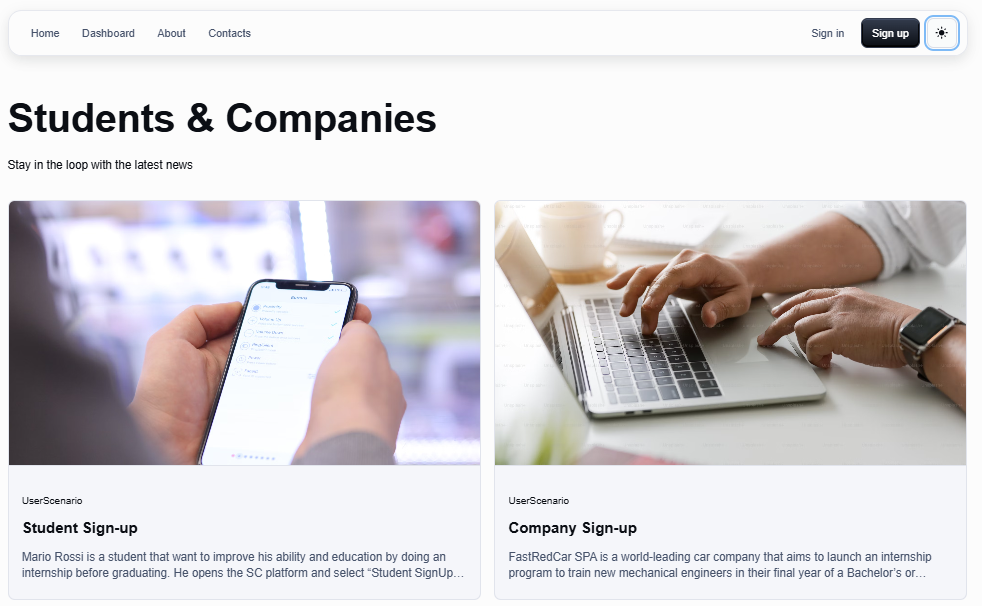
\includegraphics[width=\textwidth]{Latex/Images/HomePage.png}
    \caption{UI Home Page: as an example, UI cards containing some user scenarios described in the \ref{subsec: user scenarios}  are shown}
    \label{fig:homepage}
\end{figure}
\begin{figure}[H]
    \centering
    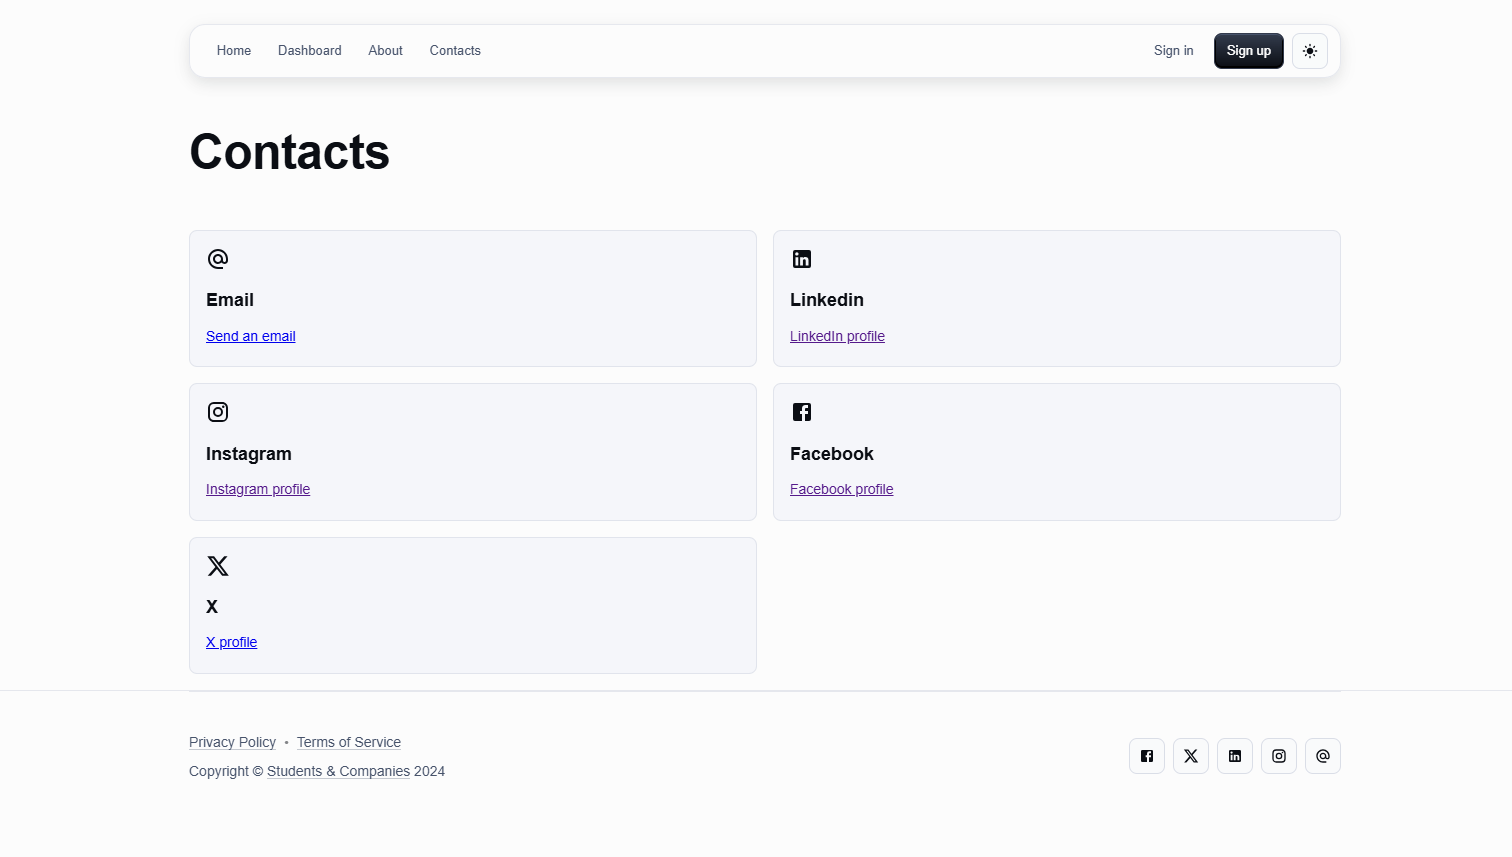
\includegraphics[width=\textwidth]{Latex/Images/New Ui/Contacts.png}
    \caption{UI Contacts Page}
    \label{fig:contactpage}
\end{figure}
\noindent Thanks to the app bar link buttons, users can also reach the Sign-Up and Sign-in pages. The Sign-Up page allows for different types of sign-up according to the new user type. This allows the user to provide the platform with the correct information.
\begin{figure}[H]
    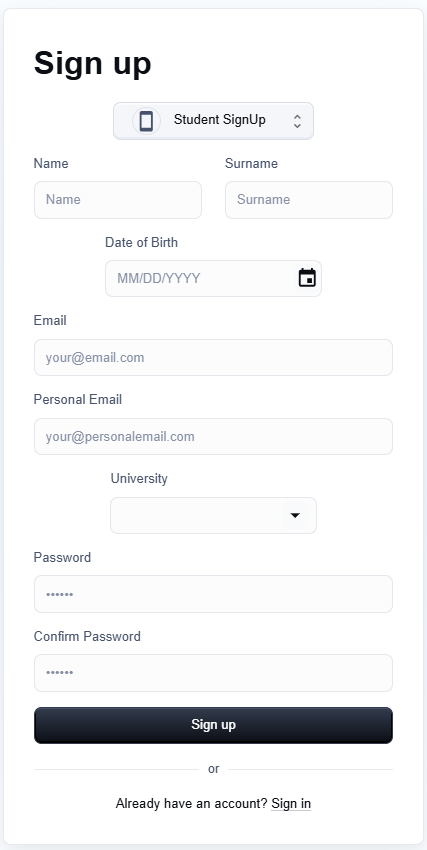
\includegraphics[width=0.33\textwidth]{Latex/Images/New Ui/SignUp Student.png}
    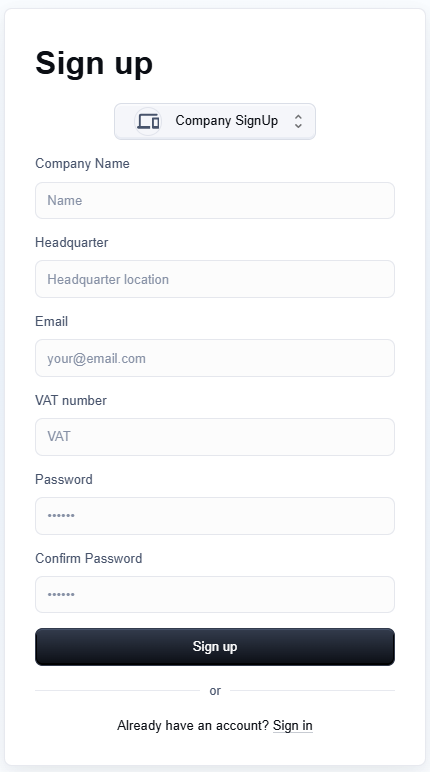
\includegraphics[width=0.33\textwidth]{Latex/Images/New Ui/SignUp Company.png}
    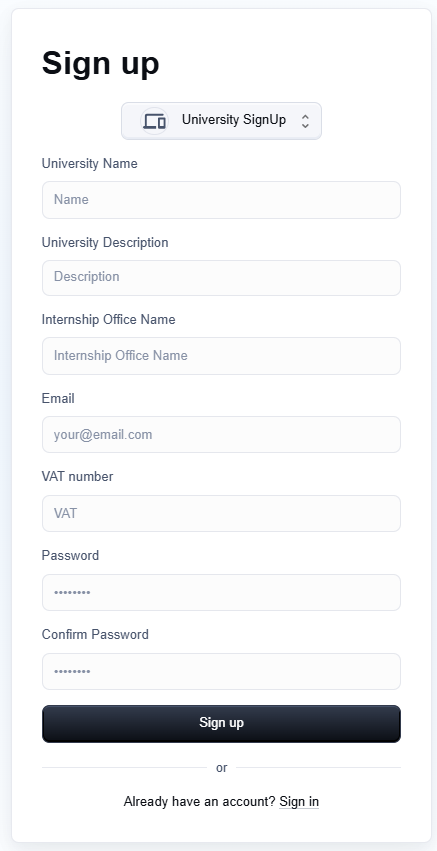
\includegraphics[width=0.33\textwidth]{Latex/Images/New Ui/SignUp University.png}
    \caption{UI Sign-Up Page}
    \label{fig:signuppage}
\end{figure}
To be able to log into the platform, the user shall provide his email and password. 
\begin{figure}[H]
    \centering
    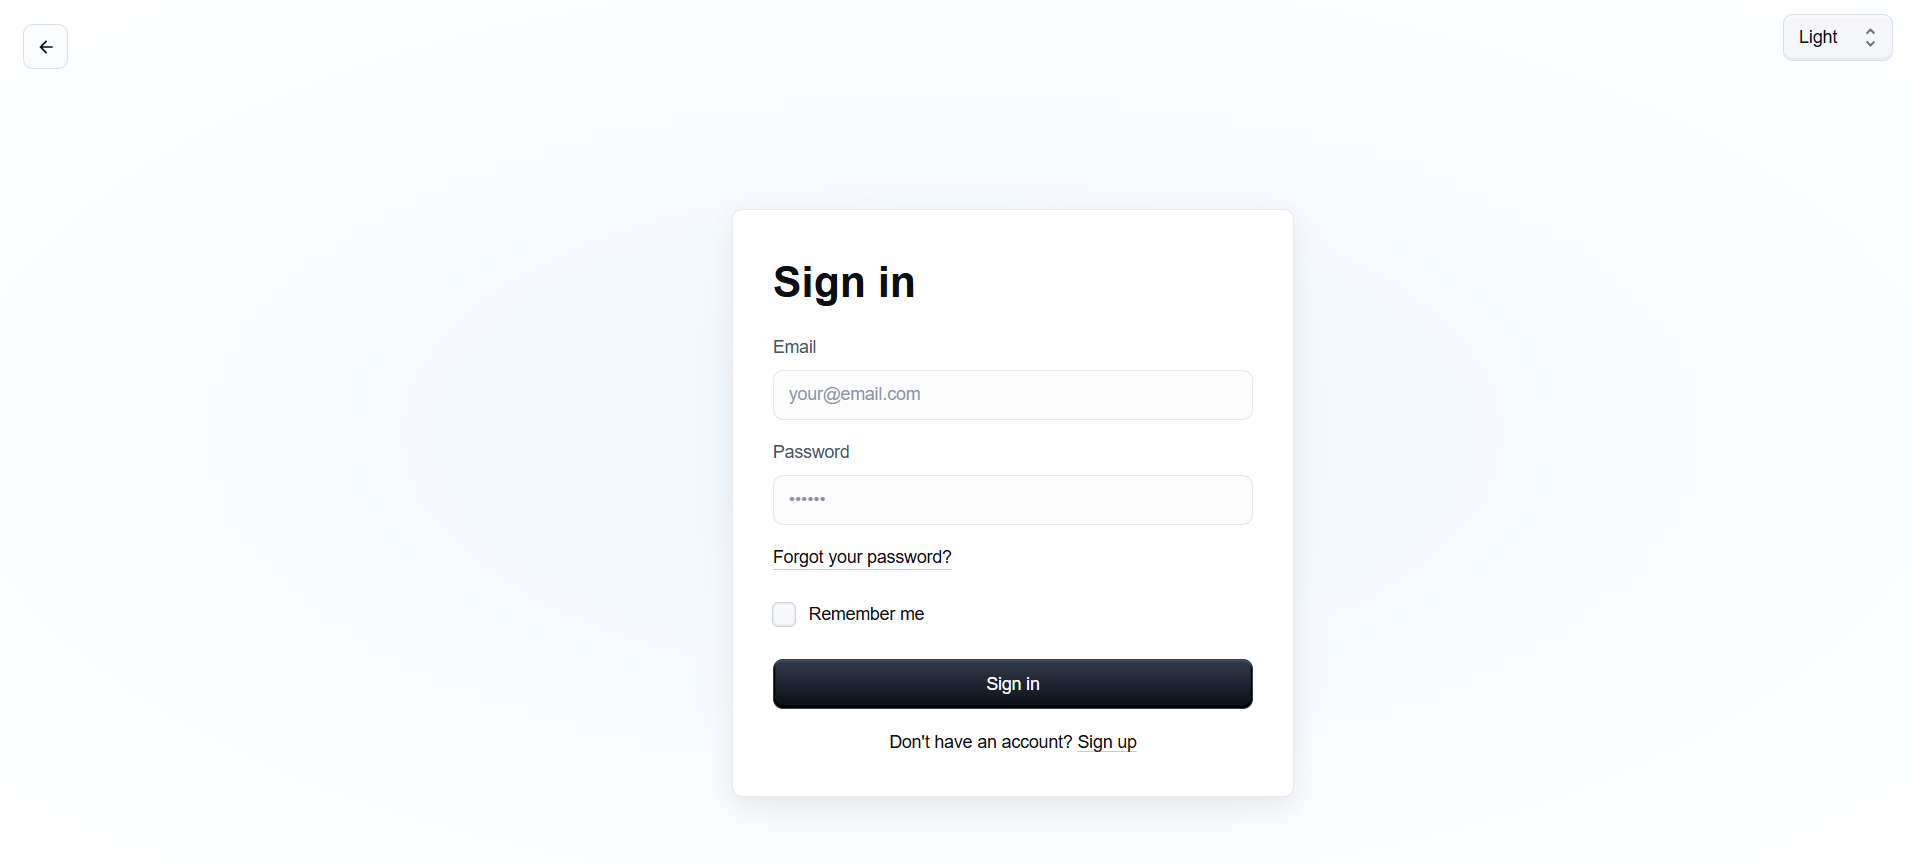
\includegraphics[width=\textwidth]{Latex/Images/New Ui/SignInPage.png}
    \caption{UI Sign-In Page}
    \label{fig:signinpage}
\end{figure}
\noindent The Dashboard page will be the central hub for logged-in users. From the left-hand panel of the dashboard, all the pages associated with the core functionalities of the platform are reachable. Therefore, this page is provided after a successful log-in. The side panel contains different elements according to the user needs.
\begin{figure}[H]
    \centering
    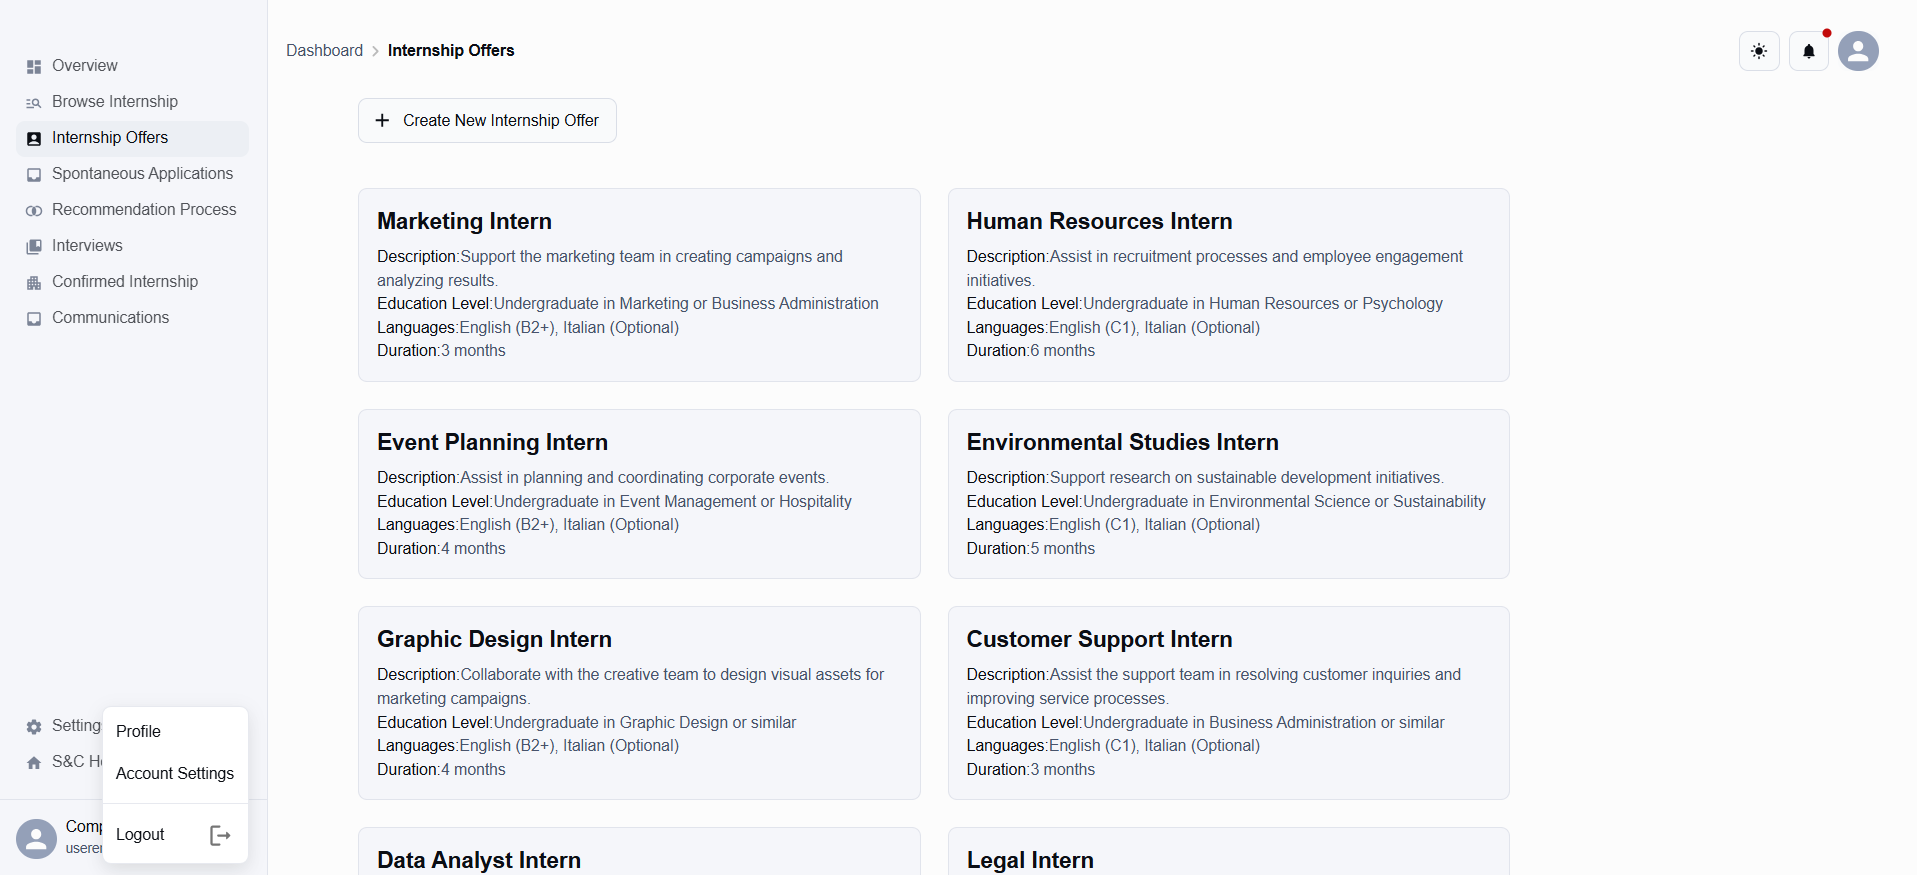
\includegraphics[width=\textwidth]{Latex/Images/New Ui/Company-Dashboard.png}
    \caption{UI Company Dashboard Page}
    \label{fig:companyDashboard}
\end{figure}
\begin{figure}[H]
    \centering
    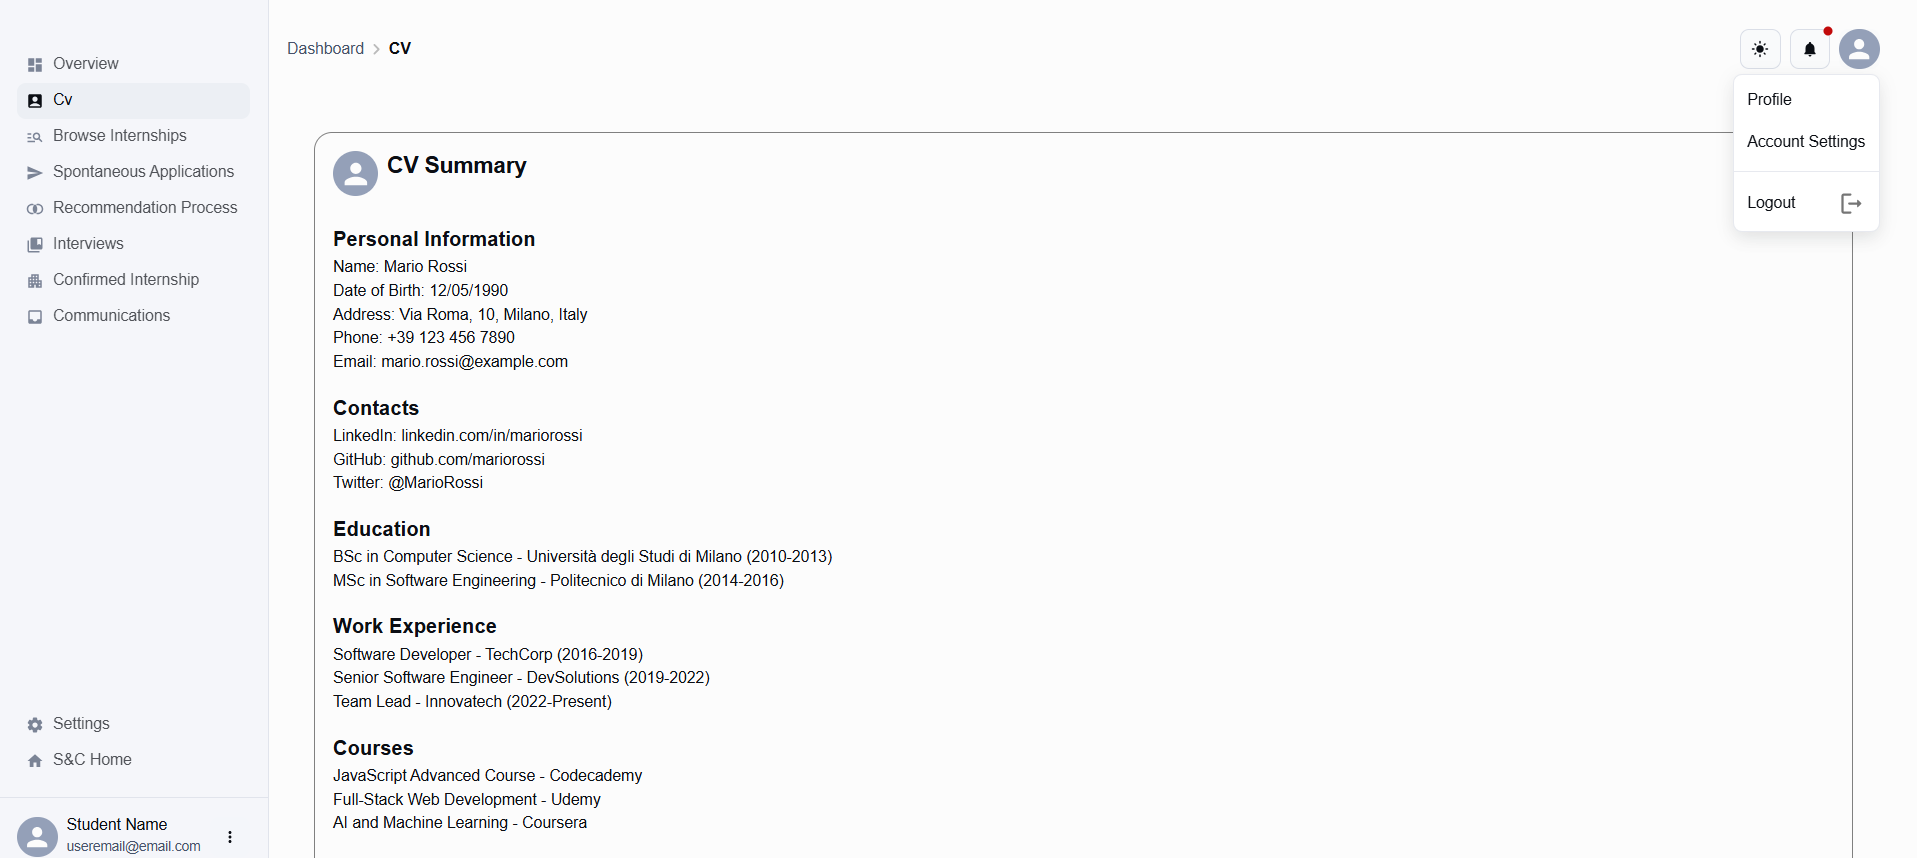
\includegraphics[width=\textwidth]{Latex/Images/New Ui/Student-Dashboard.png}
    \caption{UI Students Dashboard Page}
    \label{fig:studentDashboard}
\end{figure}
\begin{figure}[H]
    \centering
    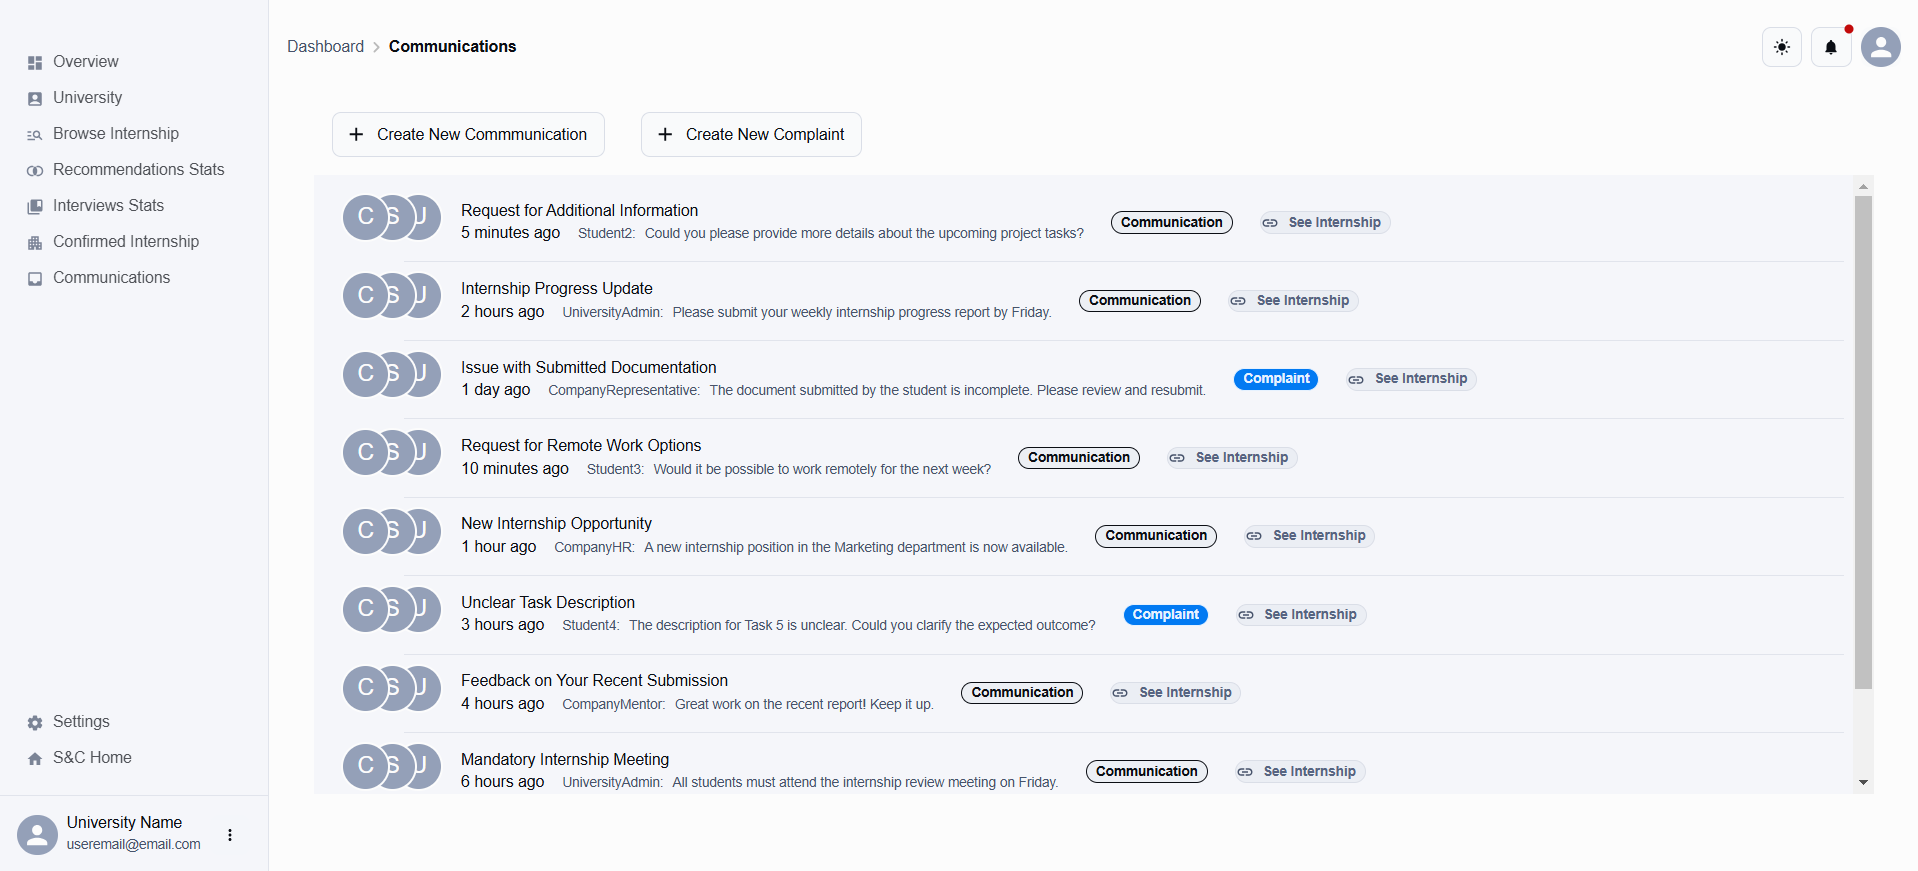
\includegraphics[width=\textwidth]{Latex/Images/New Ui/Uni-Dashboard.png}
    \caption{UI University Dashboard Page}
    \label{fig:universityDashboard}
\end{figure}
    %------------------------------------------------------------------------------------------------------------------------------------------------
    \clearpage
    \section{Requirements Traceability}
    \label{sect:req_traceability}
    

% Components list
\begin{tabular}{p{8cm} p{8cm}}
\textbf{\color{titleColor}Internal Components}  &  \textbf{\color{titleColor}External Components} \\
\begin{enumerate}[label={\color{titleColor}[C\arabic*]}]
    \item API Controller
    \item Account Manager
    \item User Manager
    \item Recommendation Process
    \item Submission Manager
    \item Interviews Manager
    \item Communication Manager
    \item Feedback Mechanism
    \item Suggestion Mechanism
    \item Platform Entity Manager
    \item Authenticator Adapter
    \item Notification Manager
    \item Notification Entity Manager
\end{enumerate}
     & 
\begin{enumerate}[label={\color{titleColor}[E\arabic*]}]
    \item Notification Provider
    \item Email Service API
    \item Authentication Provider
    \item DBMS
\end{enumerate}
\end{tabular}


% Tables for Requirement Traceability

% R1
\begin{table}[H]
    \centering
    \begin{tabular}{|p{1cm}|p{14cm}|}
    \hline
    \textbf{[R1]} & \textbf{The platform shall allow any unregistered students to register by providing personal information and selecting their University.} \\ \hline
    [C1] & API Controller \\ \hline
    [C2] & Account Manager \\ \hline
    [C10] & Platform Entity Manager \\ \hline
    [C11] & Authenticator Adapter \\ \hline
    [C12] & Notification Manager \\ \hline
    [C13] & Notification Entity Manager \\ \hline
    [E1] & Notification Provider \\ \hline
    [E2] & Email Provider API \\ \hline
    [E3] & Authentication Provider \\ \hline
    [E4] & DBMS \\ \hline
    \end{tabular}
    \caption{Requirement R1: Traceability for Student Registration Process}
    \label{tab:RT1}
\end{table}

% R2
\begin{table}[H]
    \centering
    \begin{tabular}{|p{1cm}|p{14cm}|}
    \hline
    \textbf{[R2]} & \textbf{The platform shall allow any companies to register by providing company information.} \\ \hline
    [C1] & API Controller \\ \hline
    [C2] & Account Manager \\ \hline
    [C10] & Platform Entity Manager \\ \hline
    [C11] & Authenticator Adapter \\ \hline
    [C12] & Notification Manager \\ \hline
    [C13] & Notification Entity Manager \\ \hline
    [E1] & Notification Provider \\ \hline
    [E2] & Email Provider API \\ \hline
    [E3] & Authentication Provider \\ \hline
    [E4] & DBMS \\ \hline
    \end{tabular}
    \caption{Requirement R2: Traceability for Company Registration Process}
    \label{tab:RT2}
\end{table}

% R3
\begin{table}[H]
    \centering
    \begin{tabular}{|p{1cm}|p{14cm}|}
    \hline
    \textbf{[R3]} & \textbf{The platform shall allow any universities to register by providing university information.} \\ \hline
    [C1] & API Controller \\ \hline
    [C2] & Account Manager \\ \hline
    [C10] & Platform Entity Manager \\ \hline
    [C11] & Authenticator Adapter \\ \hline
    [C12] & Notification Manager \\ \hline
    [C13] & Notification Entity Manager \\ \hline
    [E1] & Notification Provider \\ \hline
    [E2] & Email Provider API \\ \hline
    [E3] & Authentication Provider \\ \hline
    [E4] & DBMS \\ \hline
    \end{tabular}
    \caption{Requirement R3: Traceability for University Registration Process}
    \label{tab:RT3}
\end{table}

% R4
\begin{table}[H]
    \centering
    \begin{tabular}{|p{1cm}|p{14cm}|}
    \hline
    \textbf{[R4} & \textbf{The platform shall allow Users to log in using their email and password.} \\ \hline
    [C3] & User Manager \\ \hline
    [C11] & Internal Authenticator Adapter \\ \hline
    [E3] & Authentication Provider \\ \hline
    \end{tabular}
    \caption{Requirement R4: Traceability for User Login Functionality}
    \label{tab:RT4}
\end{table}

% R5
\begin{table}[H]
    \centering
    \begin{tabular}{|p{1cm}|p{14cm}|}
    \hline
    \textbf{[R5]} & \textbf{The platform shall send notifications to Users when relevant events occur.} \\ \hline
    [C12] & Notification Manager \\ \hline
    [C13] & Notification Entity Manager \\ \hline
    [E1] & Notification Provider \\ \hline
    [E4] & DBMS \\ \hline
    \end{tabular}
    \caption{Requirement R5: Traceability for Notification Functionality}
    \label{tab:RT5}
\end{table}

% R6
\begin{table}[H]
    \centering
    \begin{tabular}{|p{1cm}|p{14cm}|}
    \hline
    \textbf{[R6]} & \textbf{The platform shall allow Companies to create and publish Internship offers specifying details.} \\ \hline
    [C1] & API Controller \\ \hline
    [C3] & User Manager \\ \hline
    [C5] & Submission Manager \\ \hline
    [C10] & Platform Entity Manager \\ \hline
    [C11] & Authenticator Adapter \\ \hline
    [E3] & Authentication Provider \\ \hline
    [E4] & DBMS \\ \hline
    \end{tabular}
    \caption{Requirement R6: Traceability for Internship Offer Creation}
    \label{tab:RT6}
\end{table}

% R7
\begin{table}[H]
    \centering
    \begin{tabular}{|p{1cm}|p{14cm}|}
    \hline
    \textbf{[R7]} & \textbf{The platform shall allow Companies to terminate their Internship offers at their own discretion.} \\ \hline
    [C1] & API Controller \\ \hline
    [C3] & User Manager \\ \hline
    [C5] & Submission Manager \\ \hline
    [C10] & Platform Entity Manager \\ \hline
    [C11] & Authenticator Adapter \\ \hline
    [E3] & Authentication Provider \\ \hline
    [E4] & DBMS \\ \hline
    \end{tabular}
    \caption{Requirement R7: Traceability for Internship Termination}
    \label{tab:RT7}
\end{table}

% R8
\begin{table}[H]
    \centering
    \begin{tabular}{|p{1cm}|p{14cm}|}
    \hline
    \textbf{[R8]} & \textbf{The platform shall provide Students with Matches automatically obtained by the Recommendation Process.} \\ \hline
    [C1] & API Controller \\ \hline
    [C3] & User Manager \\ \hline
    [C4] & Recommendation Process \\ \hline
    [C10] & Platform Entity Manager \\ \hline
    [C11] & Authenticator Adapter \\ \hline
    [E3] & Authentication Provider \\ \hline
    [E4] & DBMS \\ \hline
    \end{tabular}
    \caption{Requirement R8: Traceability for Recommendation Matching}
    \label{tab:RT8}
\end{table}

% R9
\begin{table}[H]
    \centering
    \begin{tabular}{|p{1cm}|p{14cm}|}
    \hline
    \textbf{[R9]} & \textbf{The platform shall allow Students to view and navigate all available Internships.} \\ \hline
    [C1] & API Controller \\ \hline
    [C5] & Submission Manager \\ \hline
    [C10] & Platform Entity Manager \\ \hline
    [C11] & Authenticator Adapter \\ \hline
    [E3] & Authentication Provider \\ \hline
    [E4] & DBMS \\ \hline
    \end{tabular}
    \caption{Requirement R9: Traceability for Viewing Available Internships}
    \label{tab:RT9}
\end{table}

% R10
\begin{table}[H]
    \centering
    \begin{tabular}{|p{1cm}|p{14cm}|}
    \hline
    \textbf{[R10]} & \textbf{The platform shall enable Students to submit Spontaneous Applications to Internships they choose.} \\ \hline
    [C1] & API Controller \\ \hline
    [C5] & Submission Manager \\ \hline
    [C10] & Platform Entity Manager \\ \hline
    [C11] & Authenticator Adapter \\ \hline
    [E3] & Authentication Provider \\ \hline
    [E4] & DBMS \\ \hline
    \end{tabular}
    \caption{Requirement R10: Traceability for Spontaneous Applications}
    \label{tab:RT10}
\end{table}

% R11
\begin{table}[H]
    \centering
    \begin{tabular}{|p{1cm}|p{14cm}|}
    \hline
    \textbf{[R11]} & \textbf{The platform shall allow Students to submit their CV.} \\ \hline
    [C1] & API Controller \\ \hline
    [C5] & Submission Manager \\ \hline
    [C10] & Platform Entity Manager \\ \hline
    [C11] & Authenticator Adapter \\ \hline
    [E3] & Authentication Provider \\ \hline
    [E4] & DBMS \\ \hline
    \end{tabular}
    \caption{Requirement R11: Traceability for CV Submission}
    \label{tab:RT11}
\end{table}

% R12
\begin{table}[H]
    \centering
    \begin{tabular}{|p{1cm}|p{14cm}|}
    \hline
    \textbf{[R12]} & \textbf{The platform shall allow Students to modify their CV.} \\ \hline
    [C1] & API Controller \\ \hline
    [C5] & Submission Manager \\ \hline
    [C10] & Platform Entity Manager \\ \hline
    [C11] & Authenticator Adapter \\ \hline
    [E3] & Authentication Provider \\ \hline
    [E4] & DBMS \\ \hline
    \end{tabular}
    \caption{Requirement R12: Traceability for CV Modification}
    \label{tab:RT12}
\end{table}

% R13
\begin{table}[H]
    \centering
    \begin{tabular}{|p{1cm}|p{14cm}|}
    \hline
    \textbf{[R13]} & \textbf{The platform shall allow Students to monitor the status of their Spontaneous Applications.} \\ \hline
    [C1] & API Controller \\ \hline
    [C5] & Submission Manager \\ \hline
    [C10] & Platform Entity Manager \\ \hline
    [C11] & Authenticator Adapter \\ \hline
    [E3] & Authentication Provider \\ \hline
    [E4] & DBMS \\ \hline
    \end{tabular}
    \caption{Requirement R13: Traceability for Monitoring Spontaneous Applications}
    \label{tab:RT13}
\end{table}

% R14
\begin{table}[H]
    \centering
    \begin{tabular}{|p{1cm}|p{14cm}|}
    \hline
    \textbf{[R14]} & \textbf{The platform shall allow Students to monitor the status of their Recommendation.} \\ \hline
    [C1] & API Controller \\ \hline
    [C4] & Recommendation Process \\ \hline
    [C10] & Platform Entity Manager \\ \hline
    [C11] & Authenticator Adapter \\ \hline
    [E3] & Authentication Provider \\ \hline
    [E4] & DBMS \\ \hline
    \end{tabular}
    \caption{Requirement R14: Traceability for Monitoring Recommendations}
    \label{tab:RT14}
\end{table}

% R15
\begin{table}[H]
    \centering
    \begin{tabular}{|p{1cm}|p{14cm}|}
    \hline
    \textbf{[R15]} & \textbf{The platform shall display to Students all the Internships found by the Recommendation Process.} \\ \hline
    [C1] & API Controller \\ \hline
    [C4] & Recommendation Process \\ \hline
    [C10] & Platform Entity Manager \\ \hline
    [C11] & Authenticator Adapter \\ \hline
    [E3] & Authentication Provider \\ \hline
    [E4] & DBMS \\ \hline
    \end{tabular}
    \caption{Requirement R15: Traceability for Displaying Recommended Internships}
    \label{tab:RT15}
\end{table}

% R16
\begin{table}[H]
    \centering
    \begin{tabular}{|p{1cm}|p{14cm}|}
    \hline
    \textbf{[R16]} & \textbf{The platform shall display to Companies all the CVs of Matched Students obtained by the Recommendation Process.} \\ \hline
    [C1] & API Controller \\ \hline
    [C4] & Recommendation Process \\ \hline
    [C10] & Platform Entity Manager \\ \hline
    [C11] & Authenticator Adapter \\ \hline
    [E3] & Authentication Provider \\ \hline
    [E4] & DBMS \\ \hline
    \end{tabular}
    \caption{Requirement R16: Traceability for Displaying Matched Student CVs}
    \label{tab:RT16}
\end{table}


% R17
\begin{table}[H]
    \centering
    \begin{tabular}{|p{1cm}|p{14cm}|}
    \hline
    \textbf{[R17]} & \textbf{The platform shall allow Students and Companies to accept a Recommendation.} \\ \hline
    [C1] & API Controller \\ \hline
    [C4] & Recommendation Process \\ \hline
    [C10] & Platform Entity Manager \\ \hline
    [C11] & Authenticator Adapter \\ \hline
    [E3] & Authentication Provider \\ \hline
    [E4] & DBMS \\ \hline
    \end{tabular}
    \caption{Requirement R17: Traceability for Accepting Recommendations}
    \label{tab:RT17}
\end{table}

% R18
\begin{table}[H]
    \centering
    \begin{tabular}{|p{1cm}|p{14cm}|}
    \hline
    \textbf{[R18]} & \textbf{The platform shall allow Companies to accept a Spontaneous Application.} \\ \hline
    [C1] & API Controller \\ \hline
    [C4] & Recommendation Process \\ \hline
    [C10] & Platform Entity Manager \\ \hline
    [C11] & Authenticator Adapter \\ \hline
    [E3] & Authentication Provider \\ \hline
    [E4] & DBMS \\ \hline
    \end{tabular}
    \caption{Requirement R18: Traceability for Accepting Spontaneous Applications}
    \label{tab:RT18}
\end{table}

% R19
\begin{table}[H]
    \centering
    \begin{tabular}{|p{1cm}|p{14cm}|}
    \hline
    \textbf{[R19]} & \textbf{The platform shall start a Selection Process only if both the Company and the Student have accepted the Recommendation.} \\ \hline
    [C1] & API Controller \\ \hline
    [C4] & Recommendation Process \\ \hline
    [C10] & Platform Entity Manager \\ \hline
    [C11] & Authenticator Adapter \\ \hline
    [E3] & Authentication Provider \\ \hline
    [E4] & DBMS \\ \hline
    \end{tabular}
    \caption{Requirement R19: Traceability for Starting Selection Process via Recommendation}
    \label{tab:RT19}
\end{table}

% R20
\begin{table}[H]
    \centering
    \begin{tabular}{|p{1cm}|p{14cm}|}
    \hline
    \textbf{[R20]} & \textbf{The platform shall start a Selection Process only if the Company has accepted the Spontaneous Application.} \\ \hline
    [C1] & API Controller \\ \hline
    [C5] & Submission Manager \\ \hline
    [C6] & Interviews Manager \\ \hline
    [C10] & Platform Entity Manager \\ \hline
    [C11] & Authenticator Adapter \\ \hline
    [E3] & Authentication Provider \\ \hline
    [E4] & DBMS \\ \hline
    \end{tabular}
    \caption{Requirement R20: Traceability for Starting Selection Process via Spontaneous Application}
    \label{tab:RT20}
\end{table}

% R21
\begin{table}[H]
    \centering
    \begin{tabular}{|p{1cm}|p{14cm}|}
    \hline
    \textbf{[R21]} & \textbf{The platform shall allow Companies to create Interviews.} \\ \hline
    [C1] & API Controller \\ \hline
    [C6] & Interviews Manager \\ \hline
    [C10] & Platform Entity Manager \\ \hline
    [C11] & Authenticator Adapter \\ \hline
    [E3] & Authentication Provider \\ \hline
    [E4] & DBMS \\ \hline
    \end{tabular}
    \caption{Requirement R21: Traceability for Creating Interviews}
    \label{tab:RT21}
\end{table}

% R22
\begin{table}[H]
    \centering
    \begin{tabular}{|p{1cm}|p{14cm}|}
    \hline
    \textbf{[R22]} & \textbf{The platform shall allow Companies to submit Interviews to Students they have initiated a Selection Process with.} \\ \hline
    [C1] & API Controller \\ \hline
    [C6] & Interviews Manager \\ \hline
    [C10] & Platform Entity Manager \\ \hline
    [C11] & Authenticator Adapter \\ \hline
    [E3] & Authentication Provider \\ \hline
    [E4] & DBMS \\ \hline
    \end{tabular}
    \caption{Requirement R22: Traceability for Submitting Interviews}
    \label{tab:RT22}
\end{table}

% R23
\begin{table}[H]
    \centering
    \begin{tabular}{|p{1cm}|p{14cm}|}
    \hline
    \textbf{[R23]} & \textbf{The platform shall allow Students to answer Interview questions and submit them.} \\ \hline
    [C1] & API Controller \\ \hline
    [C6] & Interviews Manager \\ \hline
    [C10] & Platform Entity Manager \\ \hline
    [C11] & Authenticator Adapter \\ \hline
    [E3] & Authentication Provider \\ \hline
    [E4] & DBMS \\ \hline
    \end{tabular}
    \caption{Requirement R23: Traceability for Answering and Submitting Interviews}
    \label{tab:RT23}
\end{table}

% R24
\begin{table}[H]
    \centering
    \begin{tabular}{|p{1cm}|p{14cm}|}
    \hline
    \textbf{[R24]} & \textbf{The platform shall allow Companies to manually evaluate Interview submissions.} \\ \hline
    [C6] & Interviews Manager \\ \hline
    [C10] & Platform Entity Manager \\ \hline
    [C11] & Authenticator Adapter \\ \hline
    [E3] & Authentication Provider \\ \hline
    [E4] & DBMS \\ \hline
    \end{tabular}
    \caption{Requirement R24: Traceability for Evaluating Interview Submissions}
    \label{tab:RT24}
\end{table}


% R25
\begin{table}[H]
    \centering
    \begin{tabular}{|p{1cm}|p{14cm}|}
    \hline
    \textbf{[R25]} & \textbf{The platform shall allow Students and Companies to monitor the status of their Interviews.} \\ \hline
    [C1] & API Controller \\ \hline
    [C6] & Interviews Manager \\ \hline
    [C10] & Platform Entity Manager \\ \hline
    [C11] & Authenticator Adapter \\ \hline
    [E3] & Authentication Provider \\ \hline
    [E4] & DBMS \\ \hline
    \end{tabular}
    \caption{Requirement R25: Traceability for Monitoring Interview Status}
    \label{tab:RT25}
\end{table}

% R26
\begin{table}[H]
    \centering
    \begin{tabular}{|p{1cm}|p{14cm}|}
    \hline
    \textbf{[R26]} & \textbf{The platform shall enable Companies to complete the Interview process by submitting the final outcome to each candidate.} \\ \hline
    [C1] & API Controller \\ \hline
    [C6] & Interviews Manager \\ \hline
    [C10] & Platform Entity Manager \\ \hline
    [C11] & Authenticator Adapter \\ \hline
    [E3] & Authentication Provider \\ \hline
    [E4] & DBMS \\ \hline
    \end{tabular}
    \caption{Requirement R26: Traceability for Submitting Interview Outcomes}
    \label{tab:RT26}
\end{table}

% R27
\begin{table}[H]
    \centering
    \begin{tabular}{|p{1cm}|p{14cm}|}
    \hline
    \textbf{[R27]} & \textbf{The platform shall enable Companies to send an Internship Position Offer to a Student only if he previously passed the relative Interview.} \\ \hline
    [C1] & API Controller \\ \hline
    [C6] & Interviews Manager \\ \hline
    [C10] & Platform Entity Manager \\ \hline
    [C11] & Authenticator Adapter \\ \hline
    [E3] & Authentication Provider \\ \hline
    [E4] & DBMS \\ \hline
    \end{tabular}
    \caption{Requirement R27: Traceability for Sending Internship Position Offers}
    \label{tab:RT27}
\end{table}

% R28
\begin{table}[H]
    \centering
    \begin{tabular}{|p{1cm}|p{14cm}|}
    \hline
    \textbf{[R28]} & \textbf{The platform shall enable Students to accept or reject an Internship Position Offer sent by a Company only if he previously passed the relative Interview.} \\ \hline
    [C1] & API Controller \\ \hline
    [C6] & Interviews Manager \\ \hline
    [C10] & Platform Entity Manager \\ \hline
    [C11] & Authenticator Adapter \\ \hline
    [E3] & Authentication Provider \\ \hline
    [E4] & DBMS \\ \hline
    \end{tabular}
    \caption{Requirement R28: Traceability for Accepting or Rejecting Internship Position Offers}
    \label{tab:RT28}
\end{table}

% R29
\begin{table}[H]
    \centering
    \begin{tabular}{|p{1cm}|p{14cm}|}
    \hline
    \textbf{[R29]} & \textbf{The platform shall collect Feedback from both Students and Companies regarding the Recommendation Process.} \\ \hline
    [C1] & API Controller \\ \hline
    [C8] & Feedback Mechanism \\ \hline
    [C10] & Platform Entity Manager \\ \hline
    [C11] & Authenticator Adapter \\ \hline
    [E3] & Authentication Provider \\ \hline
    [E4] & DBMS \\ \hline
    \end{tabular}
    \caption{Requirement R29: Traceability for Collecting Feedback on Recommendation Process}
    \label{tab:RT29}
\end{table}

% R30
\begin{table}[H]
    \centering
    \begin{tabular}{|p{1cm}|p{14cm}|}
    \hline
    \textbf{[R30]} & \textbf{The platform shall provide Suggestions to Students on improving their CVs.} \\ \hline
    [C1] & API Controller \\ \hline
    [C9] & Suggestion Mechanism \\ \hline
    [C10] & Platform Entity Manager \\ \hline
    [C11] & Authenticator Adapter \\ \hline
    [E3] & Authentication Provider \\ \hline
    [E4] & DBMS \\ \hline
    \end{tabular}
    \caption{Requirement R30: Traceability for Providing CV Improvement Suggestions}
    \label{tab:RT30}
\end{table}

% R31
\begin{table}[H]
    \centering
    \begin{tabular}{|p{1cm}|p{14cm}|}
    \hline
    \textbf{[R31]} & \textbf{The platform shall provide Suggestions to Companies on improving Internship descriptions.} \\ \hline
    [C1] & API Controller \\ \hline
    [C9] & Suggestion Mechanism \\ \hline
    [C10] & Platform Entity Manager \\ \hline
    [C11] & Authenticator Adapter \\ \hline
    [E3] & Authentication Provider \\ \hline
    [E4] & DBMS \\ \hline
    \end{tabular}
    \caption{Requirement R31: Traceability for Improving Internship Descriptions}
    \label{tab:RT31}
\end{table}

% R32
\begin{table}[H]
    \centering
    \begin{tabular}{|p{1cm}|p{14cm}|}
    \hline
    \textbf{[R32]} & \textbf{The platform shall allow registered Universities to access and monitor Internship Communications related to their Students.} \\ \hline
    [C1] & API Controller \\ \hline
    [C7] & Communication Manager \\ \hline
    [C10] & Platform Entity Manager \\ \hline
    [C11] & Authenticator Adapter \\ \hline
    [E3] & Authentication Provider \\ \hline
    [E4] & DBMS \\ \hline
    \end{tabular}
    \caption{Requirement R32: Traceability for Monitoring Internship Communications by Universities}
    \label{tab:RT32}
\end{table}

% R33
\begin{table}[H]
    \centering
    \begin{tabular}{|p{1cm}|p{14cm}|}
    \hline
    \textbf{[R33]} & \textbf{The platform shall provide a dedicated space for Students and Companies to exchange Communications about the current status of an Ongoing Internship.} \\ \hline
    [C1] & API Controller \\ \hline
    [C7] & Communication Manager \\ \hline
    [C10] & Platform Entity Manager \\ \hline
    [C11] & Authenticator Adapter \\ \hline
    [E3] & Authentication Provider \\ \hline
    [E4] & DBMS \\ \hline
    \end{tabular}
    \caption{Requirement R33: Traceability for Communication Space for Ongoing Internships}
    \label{tab:RT33}
\end{table}

% R34
\begin{table}[H]
    \centering
    \begin{tabular}{|p{1cm}|p{14cm}|}
    \hline
    \textbf{[R34]} & \textbf{The platform shall allow registered Universities to handle Complaints and to interrupt an Internship at their own discretion.} \\ \hline
    [C1] & API Controller \\ \hline
    [C7] & Communication Manager \\ \hline
    [C10] & Platform Entity Manager \\ \hline
    [C11] & Authenticator Adapter \\ \hline
    [E3] & Authentication Provider \\ \hline
    [E4] & DBMS \\ \hline
    \end{tabular}
    \caption{Requirement R34: Traceability for Handling Complaints and Interrupting Internships}
    \label{tab:RT34}
\end{table}
\clearpage
The following matrix provides a compact overview of the previous tables that facilitates the identification of the key components that manage the core functions of the system.
\begin{table}[H]
    \centering
    \begin{tabular}{|c|c|c|c|c|c|c|c|c|c|c|c|c|c|c|c|c|c|}
        \hline &   
        \textbf{C1}   &
        \textbf{C2}   &
        \textbf{C3}   &
        \textbf{C4}   &
        \textbf{C5}   &
        \textbf{C6}   &
        \textbf{C7}   &
        \textbf{C8}   &
        \textbf{C9}   &  
        \textbf{C10}  &   
        \textbf{C11}  &  
        \textbf{C12}  & 
        \textbf{C13}  & 
        \textbf{E1}   &
        \textbf{E2}   & 
        \textbf{E3}   &  
        \textbf{E4} \\ \hline
        %              C1  C2  C3  C4  C5  C6  C7  C8  C9 C10 C11 C12 C13  E1  E2  E3  E4
        \textbf{R1}  & X & X &   &   &   &   &   &   &   & X & X & X & X & X & X & X & X \\ \hline
        \textbf{R2}  & X & X &   &   &   &   &   &   &   & X & X & X & X & X & X & X & X \\ \hline
        \textbf{R3}  & X & X &   &   &   &   &   &   &   & X & X & X & X & X & X & X & X \\ \hline
        \textbf{R4}  &   &   & X &   &   &   &   &   &   &   & X &   &   &   &   & X &   \\ \hline
        \textbf{R5}  &   &   &   &   &   &   &   &   &   &   &   & X & X & X &   &   & X \\ \hline
        \textbf{R6}  & X &   & X &   & X &   &   &   &   & X & X &   &   &   &   & X & X \\ \hline
        \textbf{R7}  & X &   & X & X &   &   &   &   &   & X & X &   &   &   &   & X & X \\ \hline
        \textbf{R8}  & X &   & X &   &   &   &   &   &   & X & X &   &   &   &   & X & X \\ \hline
        \textbf{R9}  & X &   &   &   & X &   &   &   &   & X & X &   &   &   &   & X & X \\ \hline
        \textbf{R10} & X &   &   &   & X &   &   &   &   & X & X &   &   &   &   & X & X \\ \hline
        \textbf{R11} & X &   &   &   & X &   &   &   &   & X & X &   &   &   &   & X & X \\ \hline
        \textbf{R12} & X &   &   &   & X &   &   &   &   & X & X &   &   &   &   & X & X \\ \hline
        \textbf{R13} & X &   &   &   & X &   &   &   &   & X & X &   &   &   &   & X & X \\ \hline
        \textbf{R14} & X &   &   & X &   &   &   &   &   & X & X &   &   &   &   & X & X \\ \hline
        \textbf{R15} & X &   &   & X &   &   &   &   &   & X & X &   &   &   &   & X & X \\ \hline
        \textbf{R16} & X &   &   & X &   &   &   &   &   & X & X &   &   &   &   & X & X \\ \hline
        \textbf{R17} & X &   &   & X &   &   &   &   &   & X & X &   &   &   &   & X & X \\ \hline
        \textbf{R18} & X &   &   & X &   &   &   &   &   & X & X &   &   &   &   & X & X \\ \hline
        \textbf{R19} & X &   &   & X &   &   &   &   &   & X & X &   &   &   &   & X & X \\ \hline
        \textbf{R20} & X &   &   &   & X & X &   &   &   & X & X &   &   &   &   & X & X \\ \hline
        \textbf{R21} & X &   &   &   &   & X &   &   &   & X & X &   &   &   &   & X & X \\ \hline
        \textbf{R22} & X &   &   &   &   & X &   &   &   & X & X &   &   &   &   & X & X \\ \hline
        \textbf{R23} & X &   &   &   &   & X &   &   &   & X & X &   &   &   &   & X & X \\ \hline
        \textbf{R24} & X &   &   &   &   & X &   &   &   & X & X &   &   &   &   & X & X \\ \hline
        \textbf{R25} & X &   &   &   &   & X &   &   &   & X & X &   &   &   &   & X & X \\ \hline
        \textbf{R26} & X &   &   &   &   & X &   &   &   & X & X &   &   &   &   & X & X \\ \hline
        \textbf{R27} & X &   &   &   &   & X &   &   &   & X & X &   &   &   &   & X & X \\ \hline
        \textbf{R28} & X &   &   &   &   &   &   &   &   & X & X &   &   &   &   & X & X \\ \hline
        \textbf{R29} & X &   &   &   &   &   &   & X &   & X & X &   &   &   &   & X & X \\ \hline
        \textbf{R30} & X &   &   &   &   &   &   &   & X & X & X &   &   &   &   & X & X \\ \hline
        \textbf{R31} & X &   &   &   &   &   &   &   & X & X & X &   &   &   &   & X & X \\ \hline
        \textbf{R32} & X &   &   &   &   &   & X &   &   & X & X &   &   &   &   & X & X \\ \hline
        \textbf{R33} & X &   &   &   &   &   & X &   &   & X & X &   &   &   &   & X & X \\ \hline
        \textbf{R34} & X &   &   &   &   &   & X &   &   & X & X &   &   &   &   & X & X \\ \hline
    \end{tabular}
    \caption{Requirements Traceability Matrix}
    \label{tab:requirements_traceability}
\end{table}
    %------------------------------------------------------------------------------------------------------------------------------------------------
    \clearpage
    \section{Implementation, Integration and Test Plan}
    \label{sect:impinttest}
        This section provides a detailed plan for the implementation, integration, and testing of the S\&C platform. The first section will describe the main concepts and ideas behind the Implementation, Integration and Test plan and the following sections will provide a description for each step of it. 
    \subsection{Plan Overview}
    The platform will be implemented, integrated and tested following a mix between a \textit{thread} and \textit{bottom-up} approach thanks to the aforementioned microservices architecture that allows different service to be implemented and tested in parallel with others.\\
    The main idea is to develop one feature of the Platform Logic at a time, whenever possible, by implementing the front-end user interface (UI) and the back-end corresponding components and the notifications they will generate. Each feature will undergo unit testing before being integrated with other components. By adopting this thread-based implementation, we can begin testing component integration early in the development process, instead of waiting for the entire Platform Logic to be completed. We believe that this approach allows us to identify and resolve integration issues at an earlier stage, minimizing the risk of significant problems arising later on.\\
    However, due to dependency constraints, not all components can be developed using this thread-based approach. For example, the Recommendation Process and Suggestion Mechanism relay to the User Manager and Platform Entity Manager. To address this, the “Implementation, Integration and Test Plan” is organized into several steps, following a bottom-up approach dividing components into groups that can be developed, tested, and integrated independently.
    \subsection{Plan Stage}
    \subsubsection{Stage 1: User Manager and Notification Manager}
    In the first stage, we will develop the User Manager and part of the Notification Manager, enabling each component to store and retrieve data from its respective database. This process will also involve developing the Platform Entity Manager and the Notification Entity Manager so that each can interact with its own database. To test these two components, we will create an API controller DRIVER and a Manager DRIVER to simulate API controller calls and the various invocations from other components within the Platform Logic.\\ 
    \begin{figure}[H]
    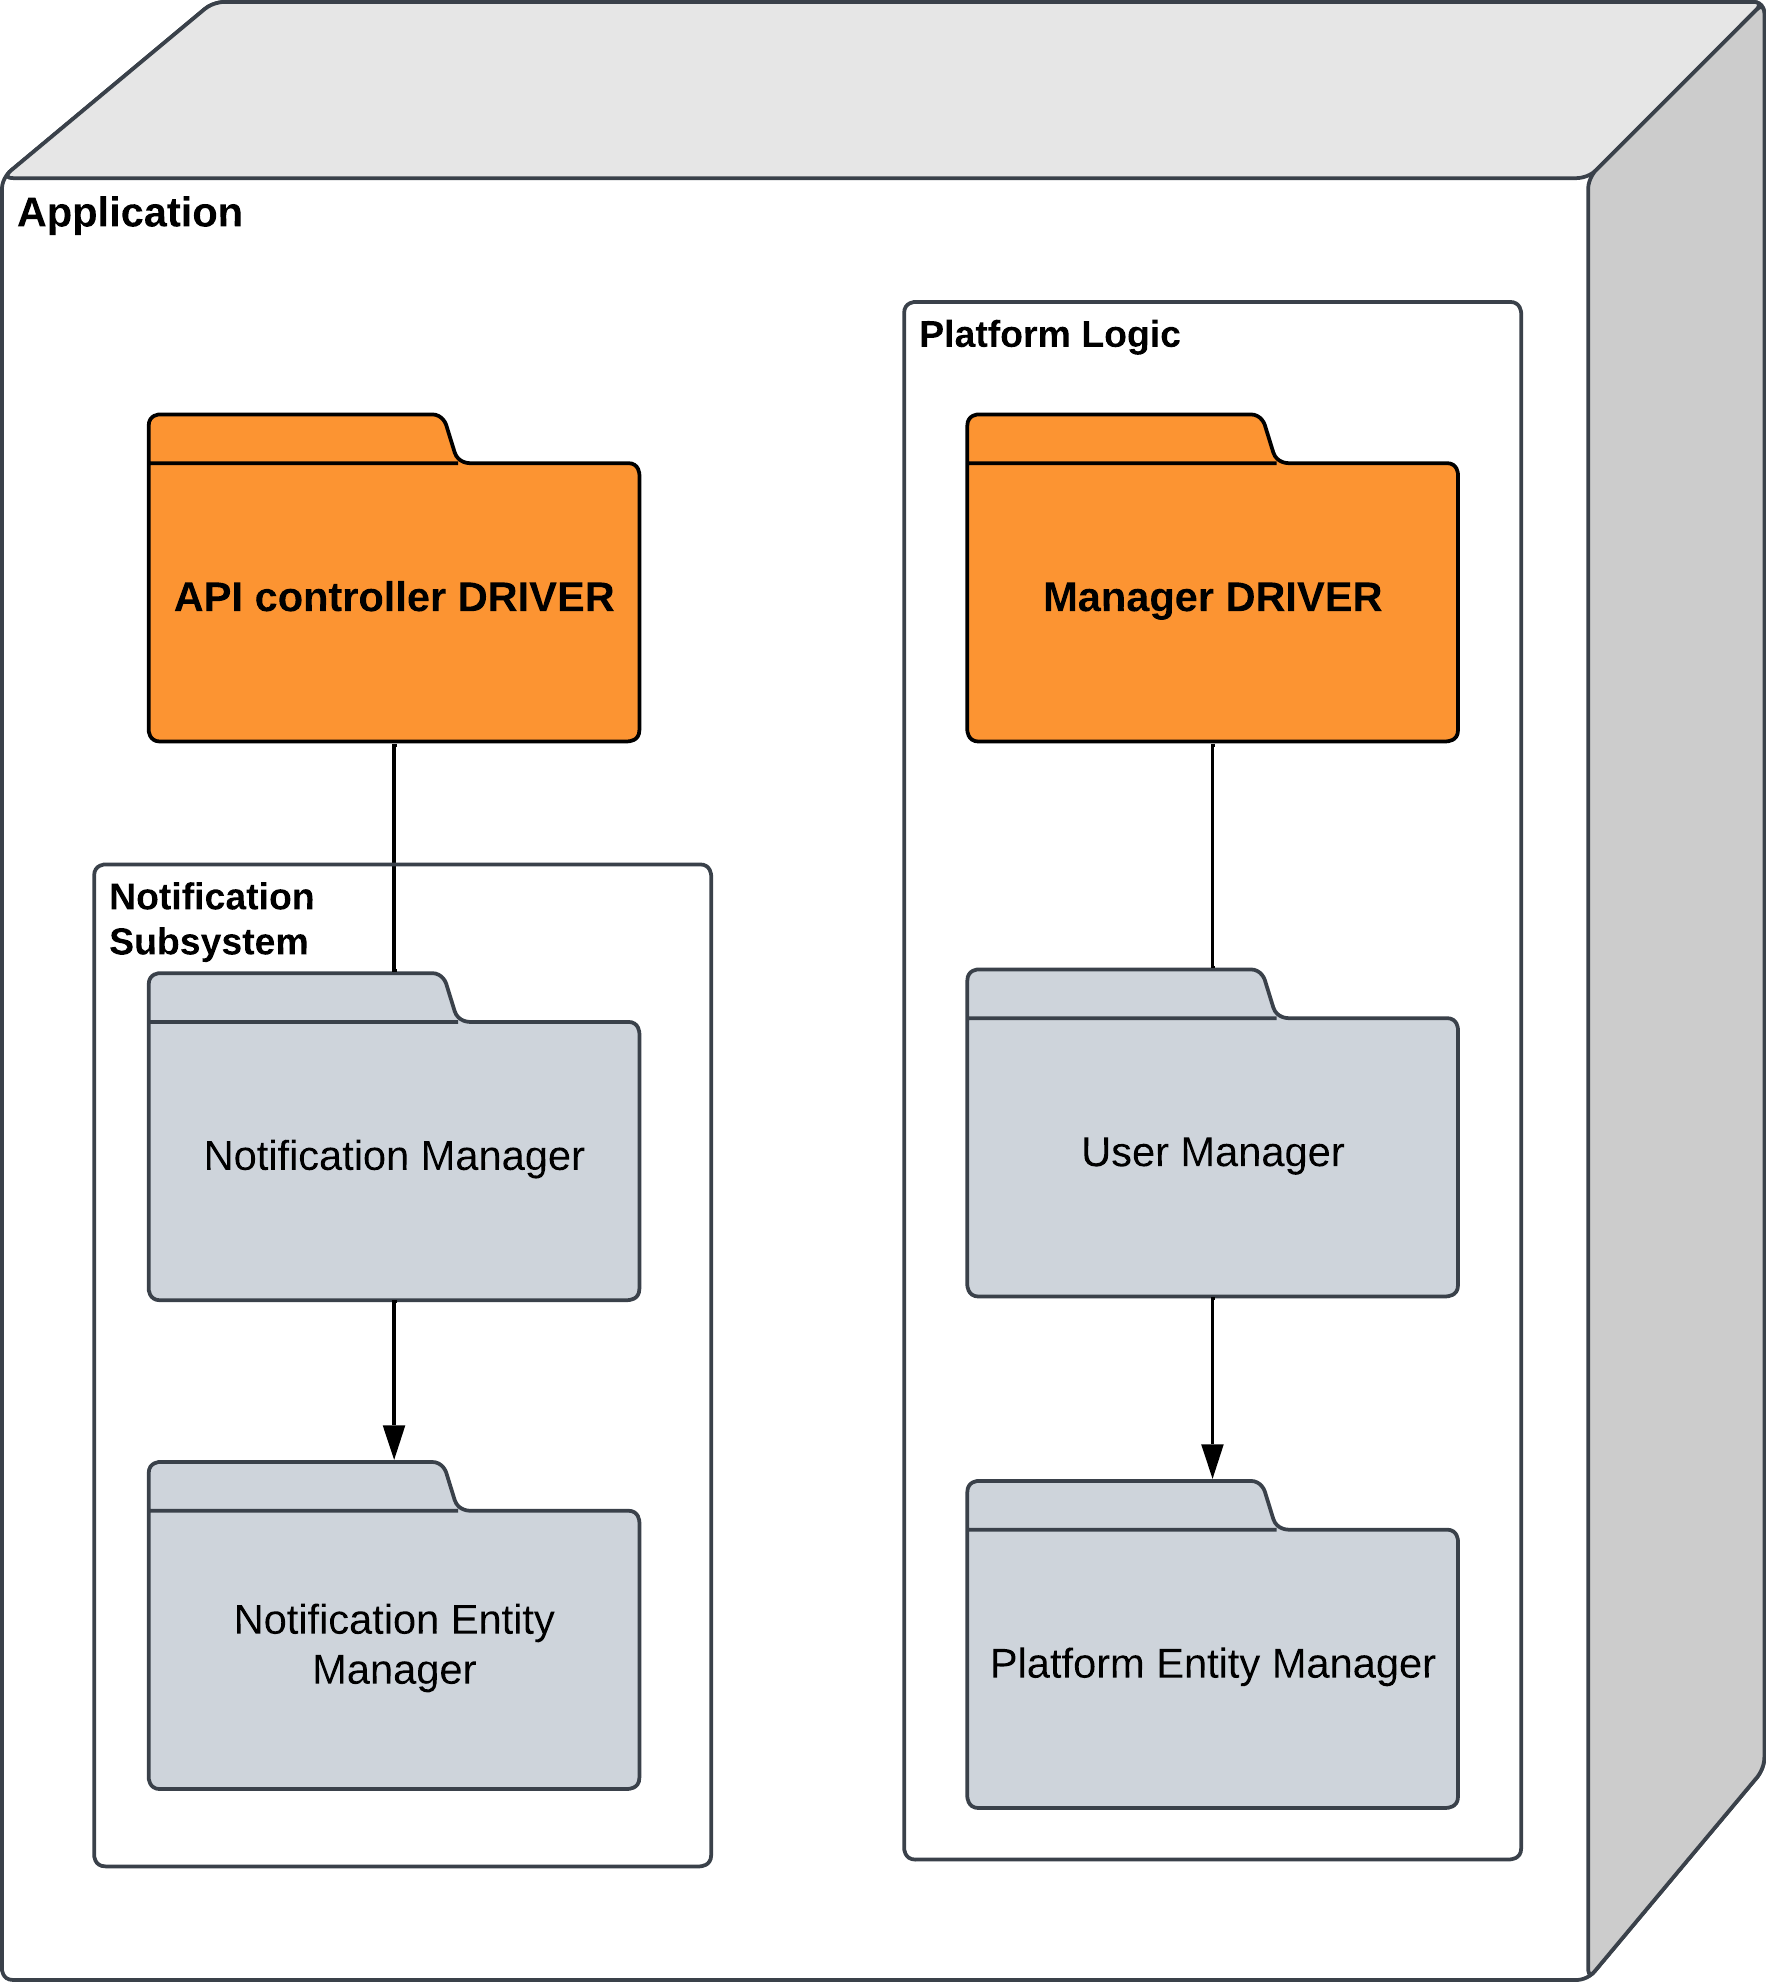
\includegraphics[width=0.35\linewidth]{Latex/Images/DD/Testing/TestingPlanStep1.png}
    \centering
    \caption{User Manager and Notification Manager testing}
    \label{fig:test-step1}
    \end{figure}
    
    \subsubsection{Stage 2: Platform Logic Components and User Interface}
    In the second stage, we will develop the remaining Platform Logic components, including the Recommendation Process, Mechanism components, and the remaining Managers. During this phase, we will also implement the User Interface (UI) and update the Notification Manager to handle notifications sent by these components, following the idea behind the \textit{thread} approach. To test these back-end components, we will create an API Controller DRIVER to simulate their invocation, while creating a Rest API STUB to simulate the front-end calls.\\
    \begin{figure}[H]
    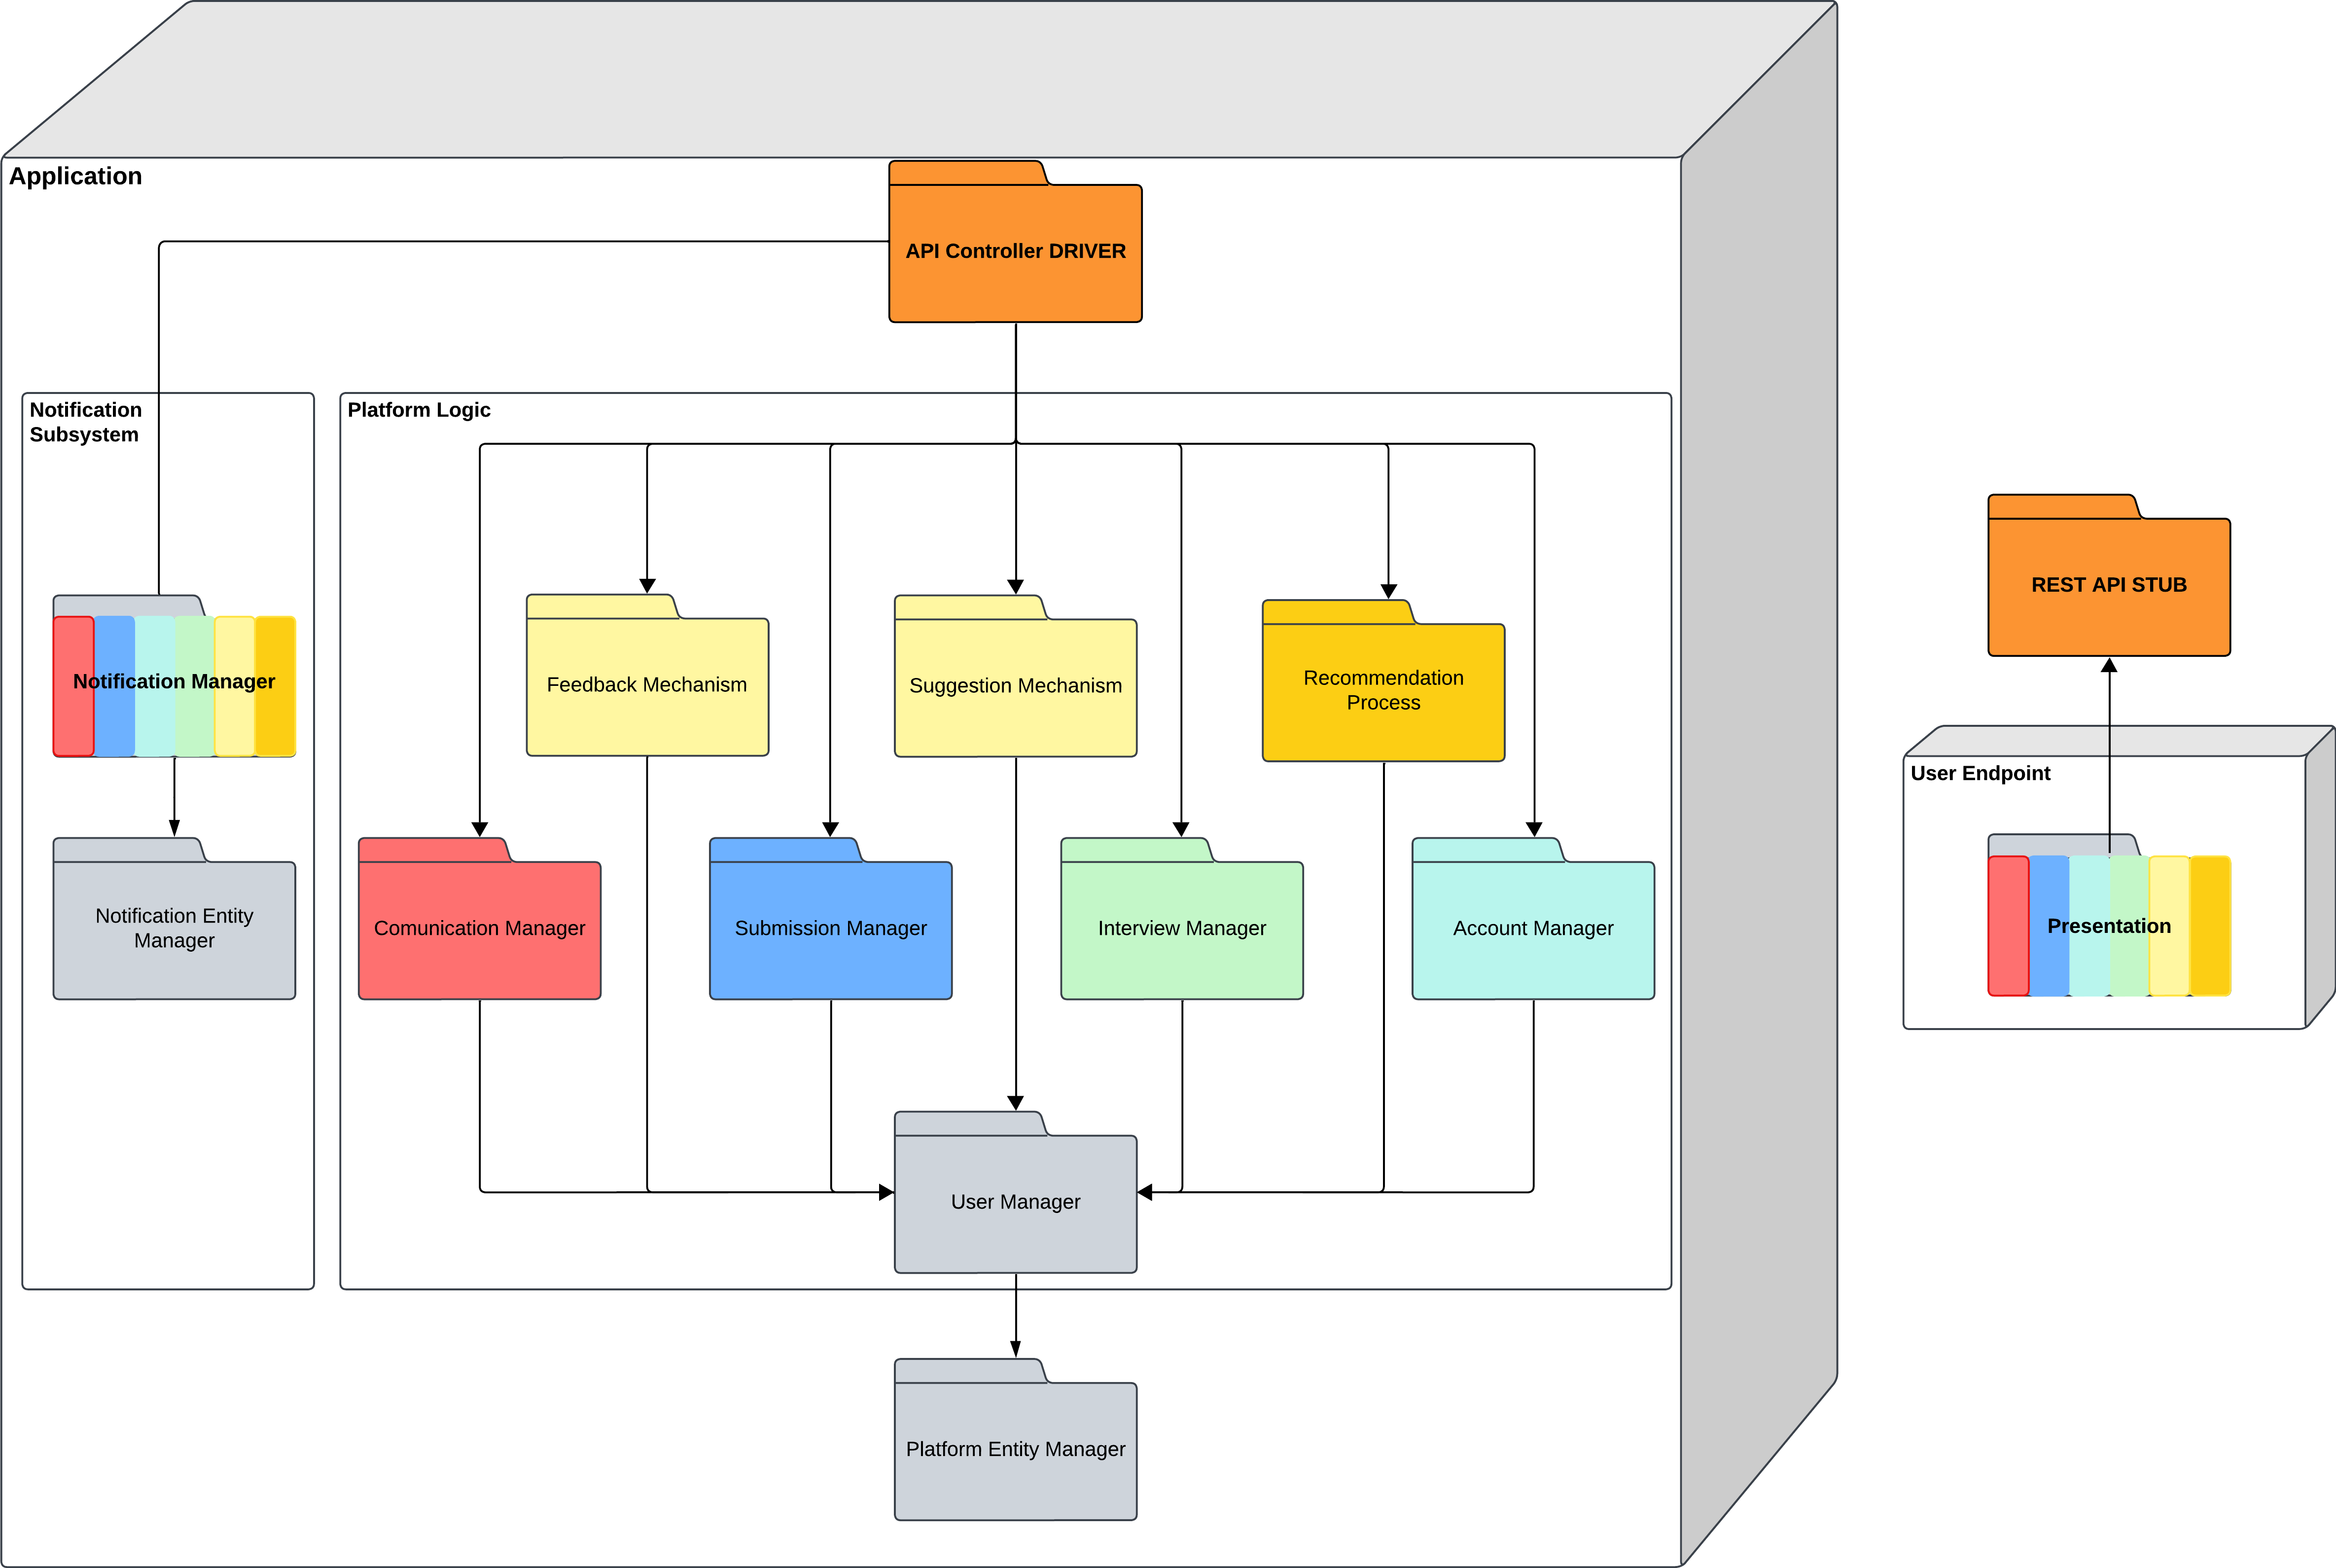
\includegraphics[width=\linewidth]{Latex/Images/DD/Testing/TestingPlanStep2.png}
    \caption{Platform Logic Components and User Interface testing}
    \label{fig:test-step2}
    \end{figure}
    
    \clearpage
    \subsubsection{Stage 3: API Controller and Front-End Integration}
    In the third stage, we will develop and integrate the API Controller with the Platform Logic components, the Notification Manager, and the User Interface that should have been completed in the previous stages. This will allow us to test the API Controller and the Platform Logic components together, ensuring that they interact correctly and that the API Controller can handle requests from the front-end and route them to the appropriate components.\\
    We will also develop the Authenticator Adapter to handle user authentication and token generation. For testing purpose we will create a Proxy DRIVER to simulate the API Controller and Authenticator Adapter calls and the front-end when it receives different responses.\\ 
    \begin{figure}[H]
    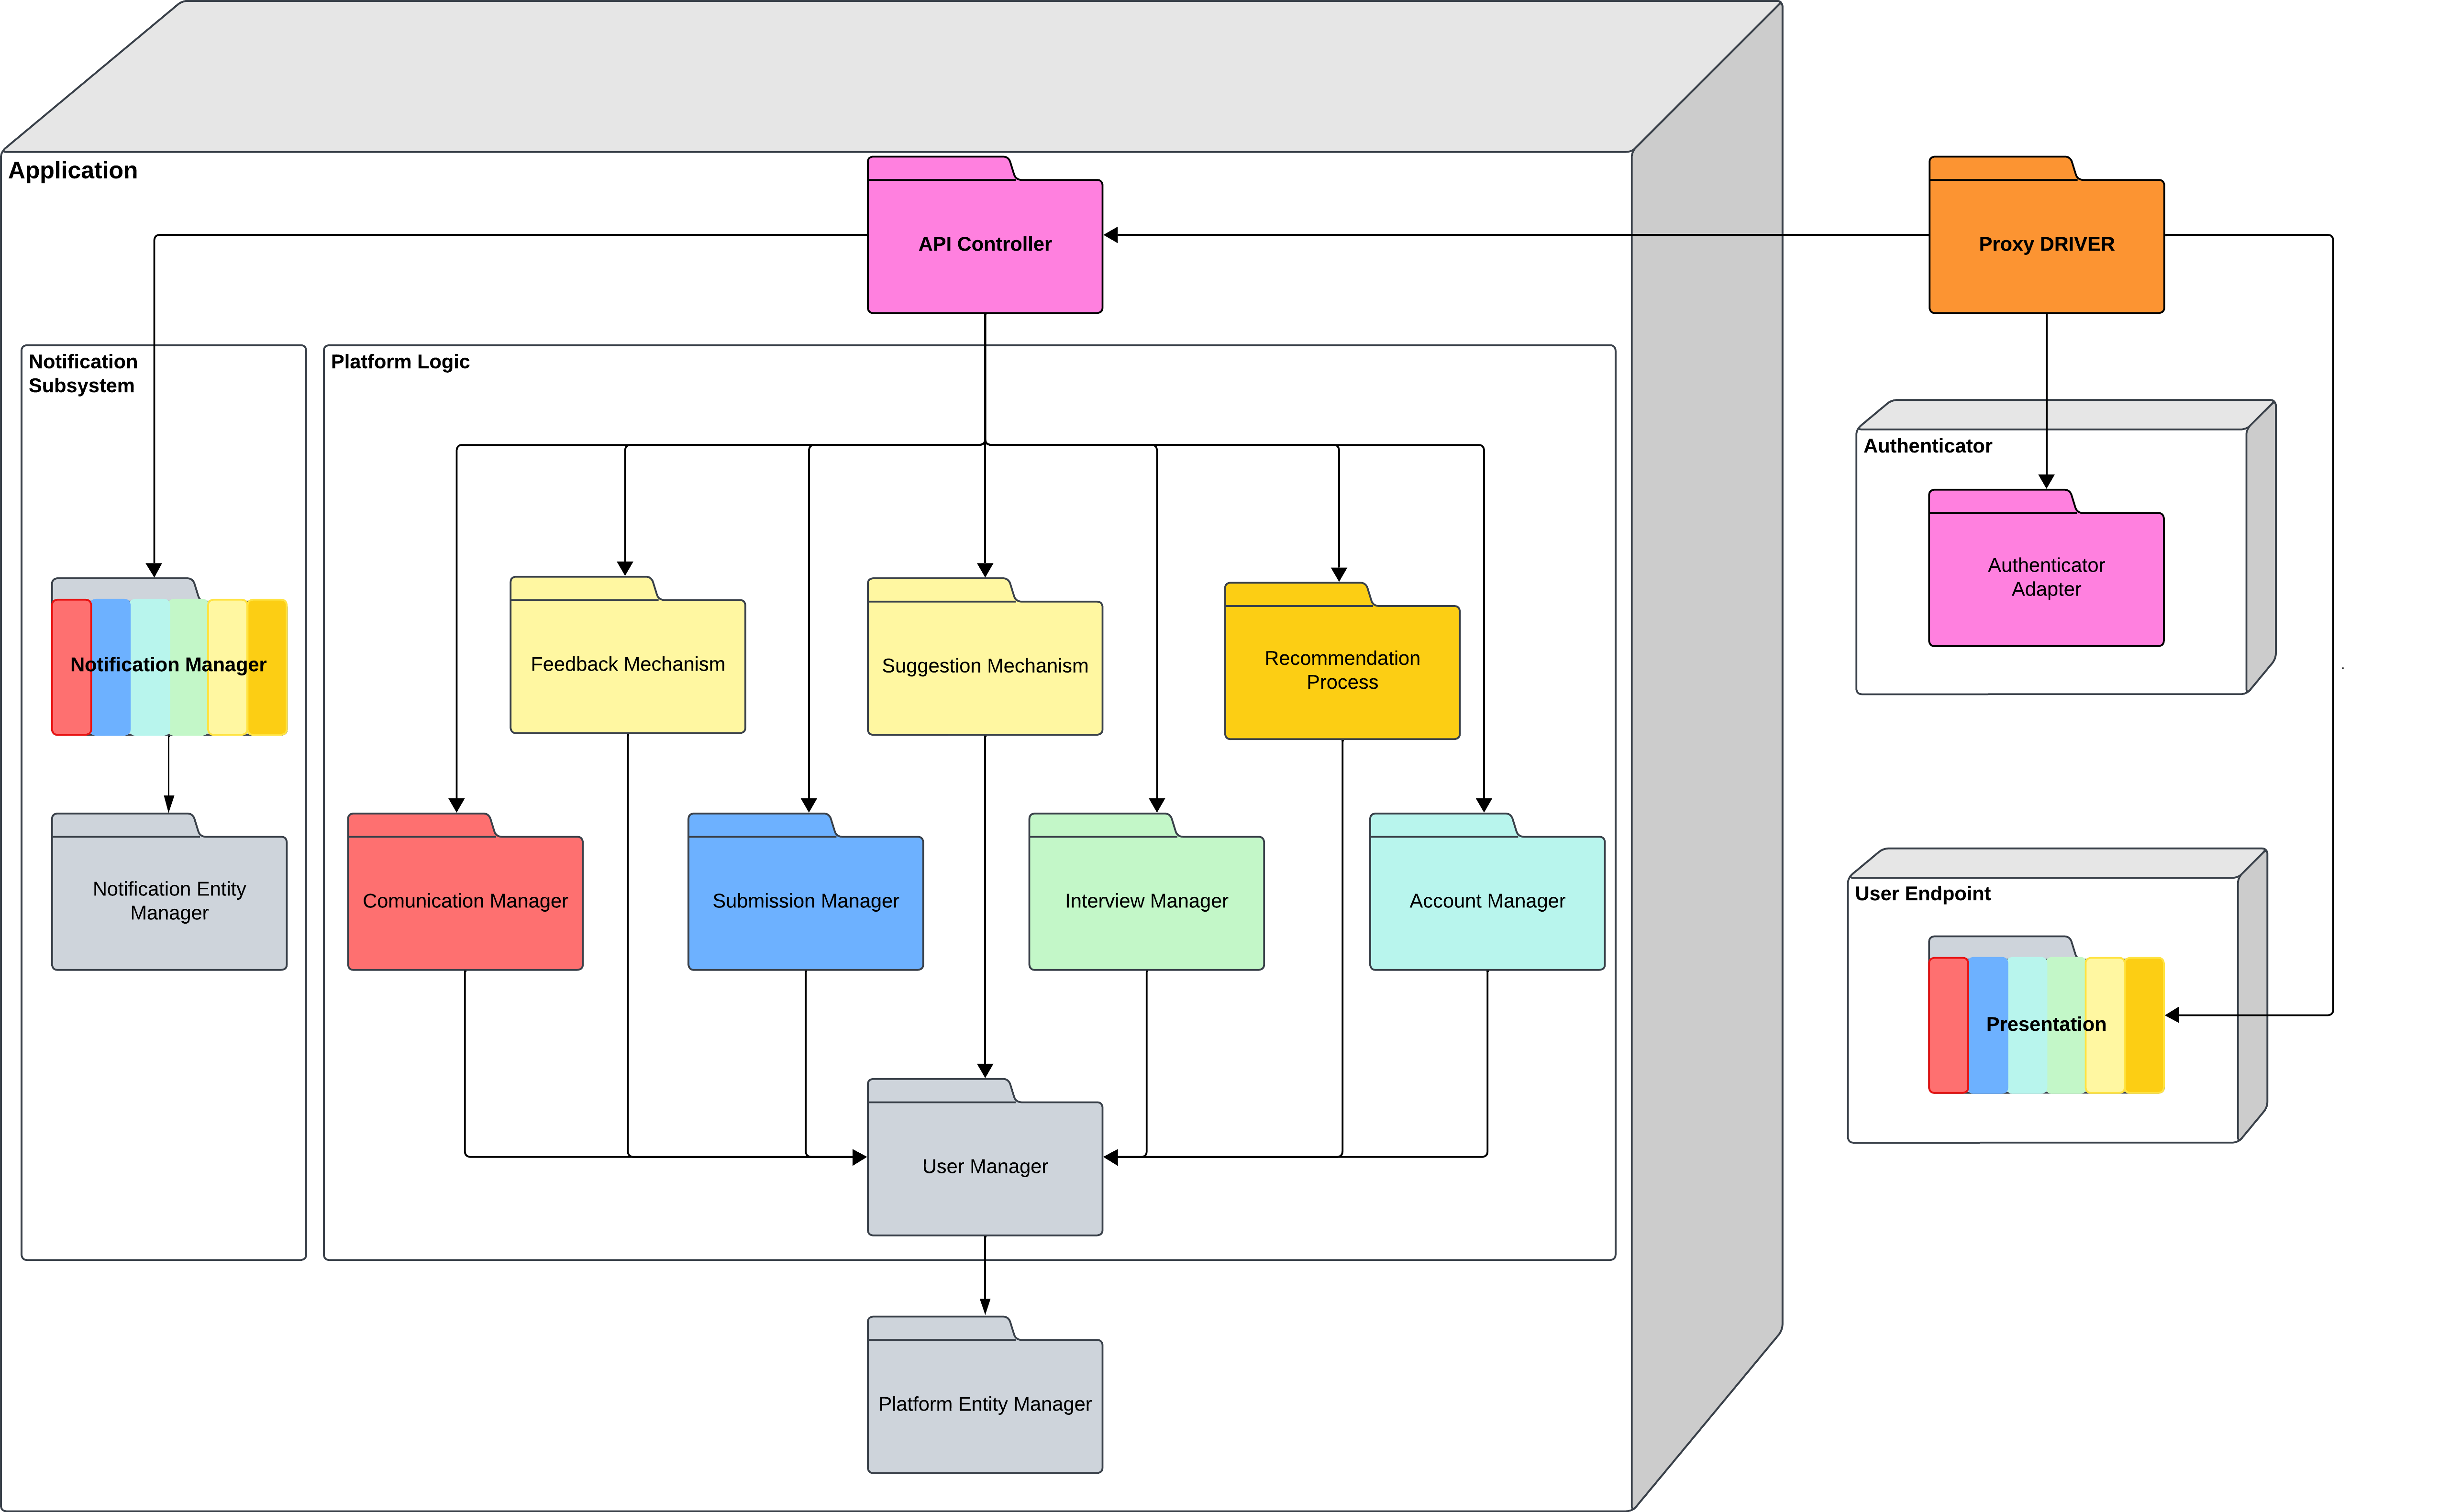
\includegraphics[width=\linewidth]{Latex/Images/DD/Testing/TestingPlanStep3.png}
    \caption{API Controller and Front-End Integration testing}
    \label{fig:test-step3}
    \end{figure}
    
    \clearpage
    \subsubsection{Stage 4: Full Integration and Testing}
    In the final stage, we will integrate all components of the platform thanks to the development of the Proxy and the Authenticator Adapter. This allows us to test the platform as a whole, ensuring that all components work together as expected. We will also conduct end-to-end testing to verify that the platform meets all requirements and functions correctly.
    \begin{figure}[H]
    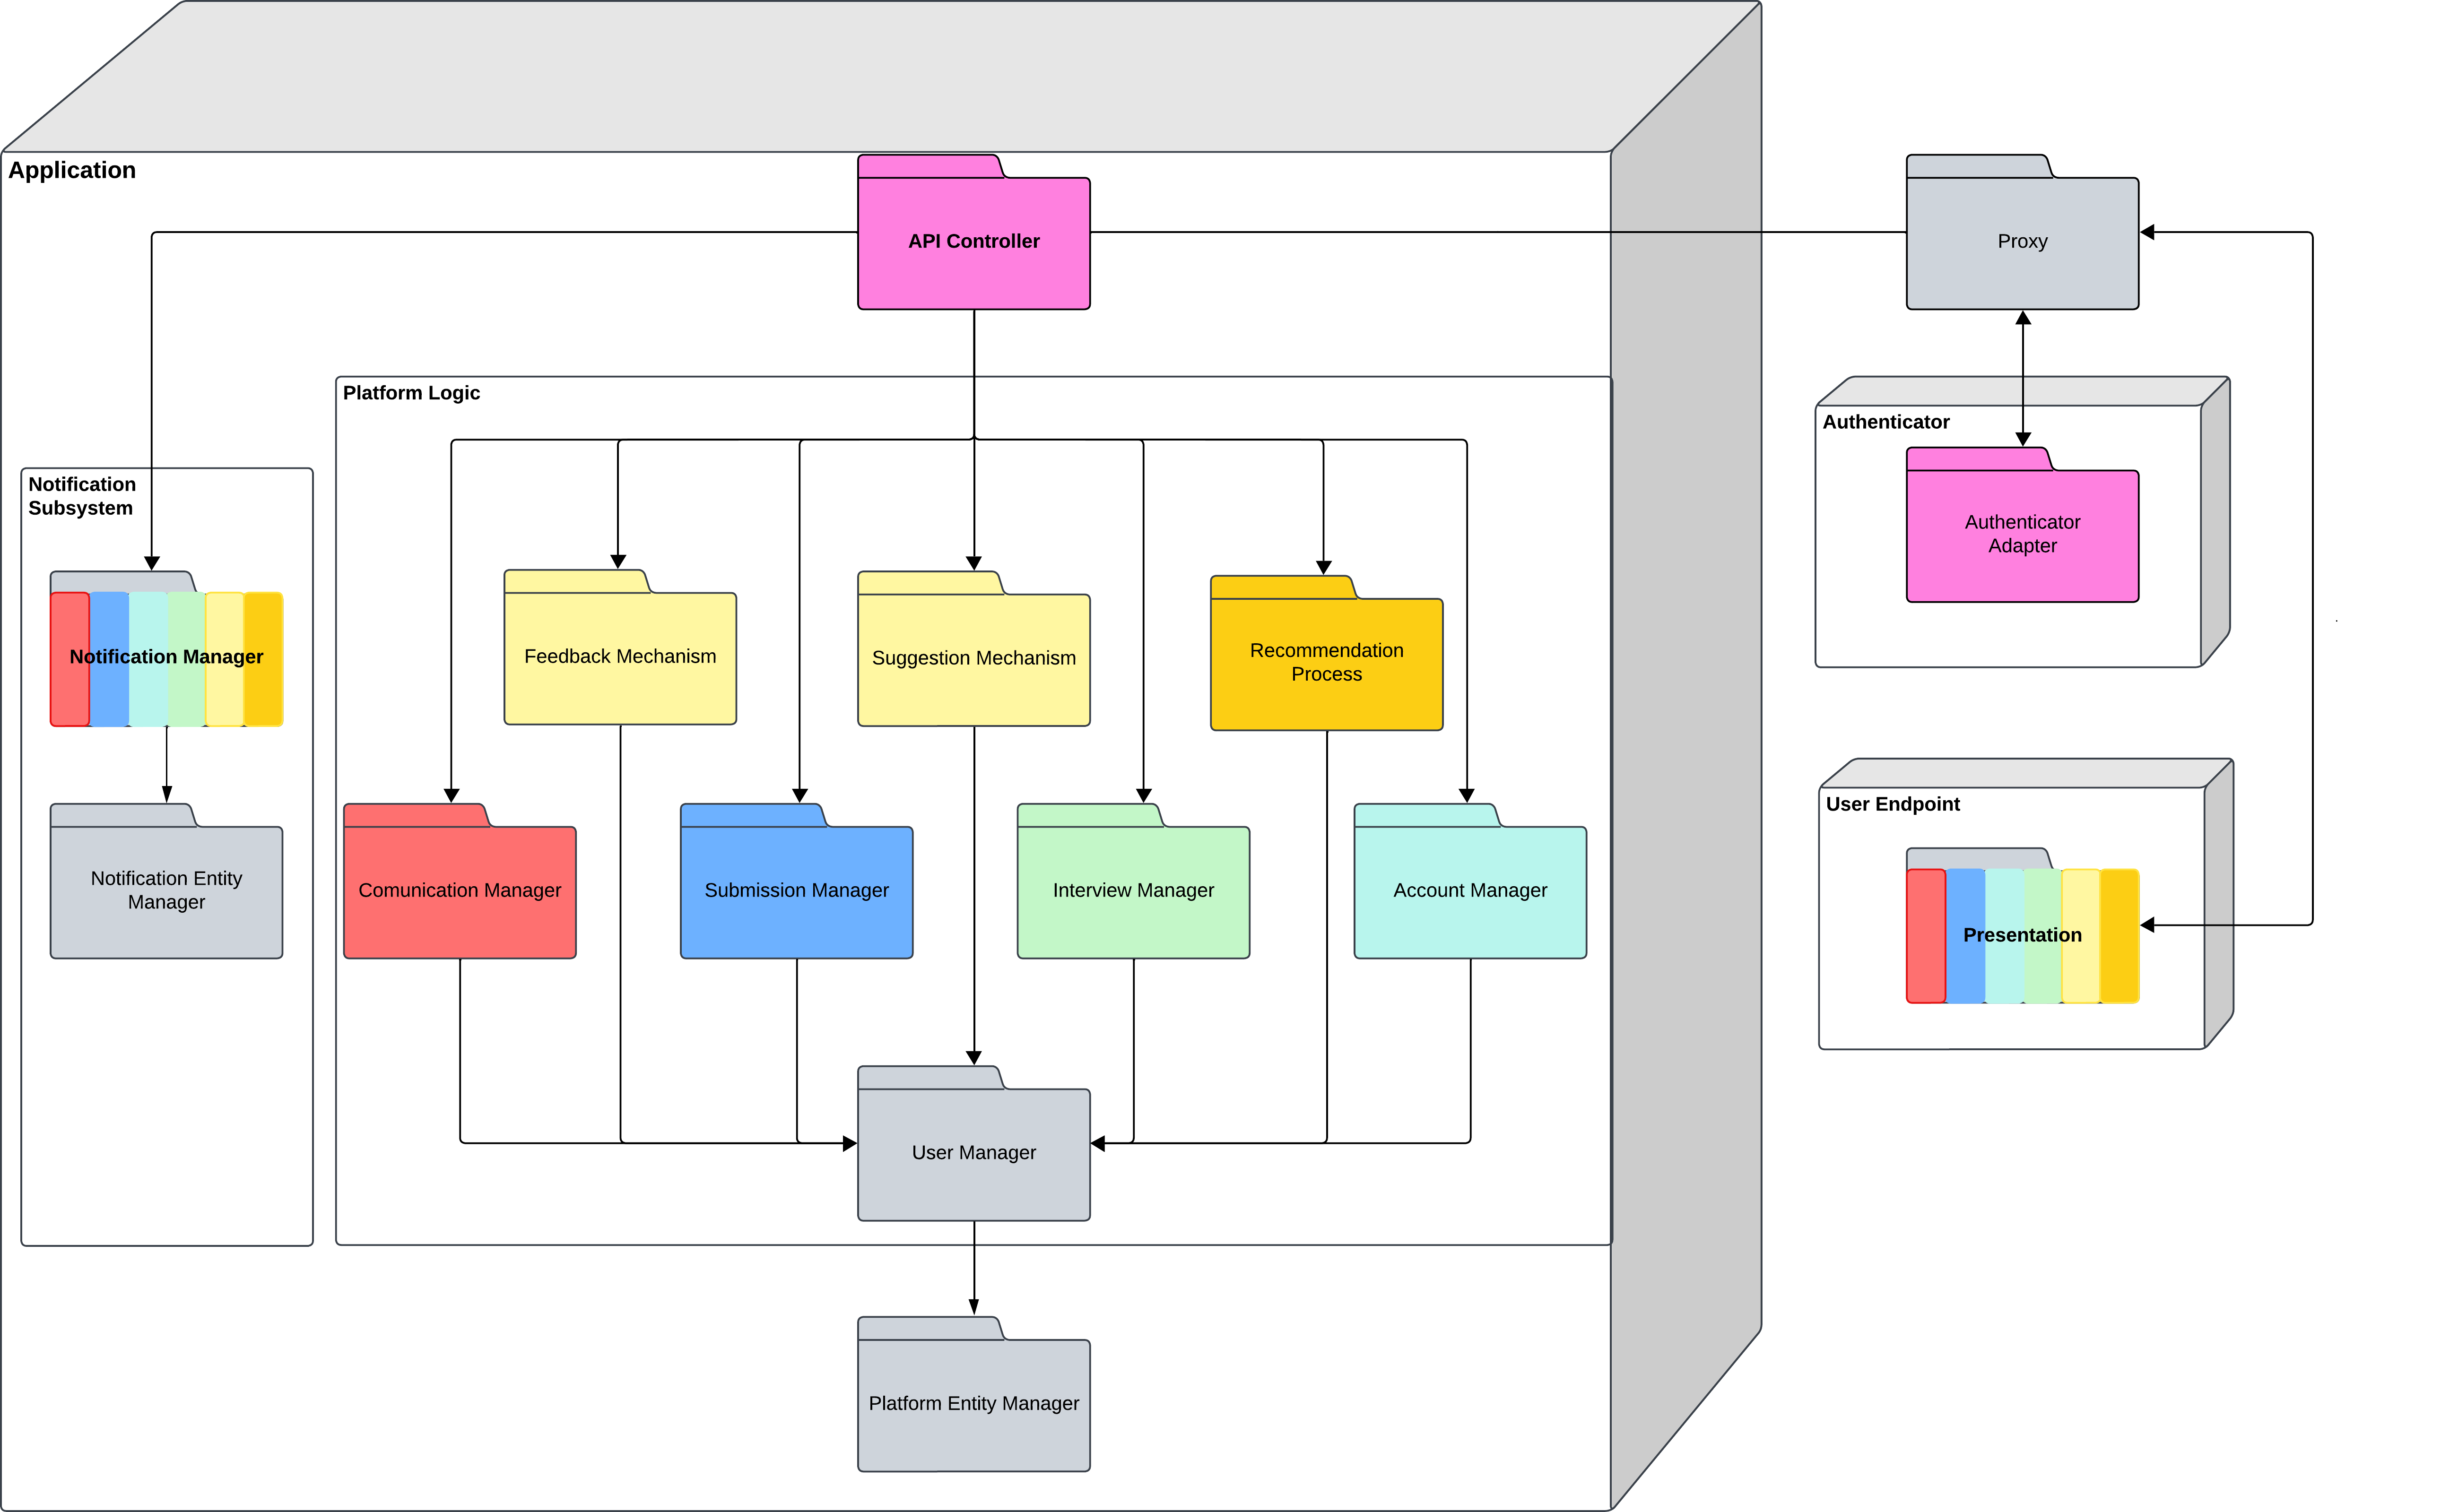
\includegraphics[width=\linewidth]{Latex/Images/DD/Testing/TestingPlanStep4.png}
    \caption{Full Integration and Testing}
    \label{fig:test-step4}
    \end{figure}
    \subsection{Technologies Used}
    In this last paragraph, we will describe the technologies used for the implementation, integration, and testing of the S\&C platform, discussing the reasons behind their choice and how they will be used in the development process.\\
    \subsubsection{Implementation Technologies}
    \begin{itemize}
        \item \textbf{Front-End}: The front-end of the platform will be developed using React, a popular JavaScript library for building user interfaces. React was chosen for its ease of use, flexibility, and performance, and wide support and documentation given the large community of developers that use it. The front-end will be styled using the MUI library to ensure a consistent and modern design across all pages and animated using the Framer Motion library.
        \item \textbf{Back-End}: The back-end of the platform will be developed using Java and Spring Boot, a popular framework for building Java-based web applications. Spring Boot was chosen robustness, and scalability, and the familiarity of the team with the Java language.
        \item \textbf{Database}: The platform's database will be established with MariaDB, a widely-used and open-source relational database management system. To engage with the database, we will utilize the Java Persistence API (JPA) alongside Hibernate, a object-relational mapping (ORM) framework for Java applications, which enables us to handle the data without manually crafting SQL queries.
        \item \textbf{Authentication}: Firebase Authentication, a reliable and popular service from Google, will be utilized to implement the authentication system for the platform. Firebase Auth was selected due to its easy of integration, scalability, and the range of authentication options it offers, such as email/password and logins via popular social networks like Facebook or Google.\\
        Moreover, Firebase Auth offers inherent security functionalities, including token-based authentication and secure user management, which correspond with our platform's requirement to manage sensitive information securely and efficiently
        \item \textbf{Notifications}: The platform’s notification system will be built with Firebase Cloud Messaging (FCM), a cross-platform messaging service that enables us to deliver push notifications to users on Android, iOS, and the web. FCM was selected for its dependability, scalability, and seamless integration with Firebase Auth, enabling us to send notifications securely and efficiently to platform users.
    \end{itemize}
    \subsubsection{Integration and Testing Technologies}
    \begin{itemize}
        \item \textbf{Unit Testing}: The platform's components of the back end will be tested using JUnit, a popular unit testing framework for Java applications.\\
        Moreover, JUnit was chosen for its simplicity, ease of use, compatibility with the Spring Boot framework and the team's familiarity with the tool.
        \item \textbf{Back-end Mock}: Mockito, a widely-used mocking framework for Java applications, will be used to create stub and mock objects for testing purposes.\\
        Moreover, Mockito was selected for its flexibility, ease of use, and compatibility with JUnit, allowing us both to simulate the behavior of external dependencies and to verify the interactions between components.
        \item \textbf{Front-end Testing}: The front-end of the platform will be tested using React Testing Library, a popular testing utility for React applications.\\
        Moreover, React Testing Library was chosen for the same reasons as React, and it allows us to write tests that closely resemble how users interact with the application, ensuring that the UI functions as expected.
        \item \textbf{Front-end Mock}: MSW (Mock Service Worker) will be used to mock the API calls made by the front-end during testing.\\
        Moreover, MSW was chosen for its ease of use, flexibility, and compatibility with React Testing Library, enabling us to simulate the behavior of the back-end components and test the front-end in isolation. 
    \end{itemize}
    
    %------------------------------------------------------------------------------------------------------------------------------------------------
    \clearpage
    \section{Effort Spent}
    \label{sect:effort}
    \subsection*{Lorenzo Ricci}
\begin{table}[H]
    \centering
\begin{tabular}{|l|c|}
        \hline
        \textbf{Section} & \textbf{Hours} \\ \hline
        Introduction & 3 \\ \hline
        Architectural Design & 20 \\ \hline
        User Interface Design & 2 \\ \hline
        Requirements Traceability & 1\\ \hline
        Implementation, Integration, and Test Plan & 2 \\ \hline
        Misc Activities & 15 \\ \hline
    \end{tabular}
    \caption{Effort - Lorenzo Ricci}
    \label{tab:effortricci}
\end{table}
\subsection*{Matteo Giovanni Paoli}
\begin{table}[H]
    \centering
\begin{tabular}{|l|c|}
        \hline
        \textbf{Section} & \textbf{Hours} \\ \hline
        Introduction & 2 \\ \hline
        Architectural Design & 24 \\ \hline
        User Interface Design & 0.5 \\ \hline
        Implementation, Integration, and Test Plan & 4 \\ \hline
        Misc Activities & 0 \\ \hline
    \end{tabular}
    \caption{Effort - Matteo Giovanni Paoli}
    \label{tab:effortpaoli}
\end{table}
\subsection*{Samuele Grisoni}
\begin{table}[H]
    \centering
\begin{tabular}{|l|c|}
        \hline
        \textbf{Section} & \textbf{Hours} \\ \hline
        Introduction & 6 \\ \hline
        Architectural Design & 20 \\ \hline
        User Interface Design & 1 \\ \hline
        Requirements Traceability & 1\\ \hline
        Implementation, Integration, and Test Plan & 5 \\ \hline
        Misc Activities & 3\\ \hline
    \end{tabular}
    \caption{Effort - Samuele Grisoni}
    \label{tab:effortgrisoni}
\end{table}
    %------------------------------------------------------------------------------------------------------------------------------------------------
    \clearpage
    \section{References}
    \label{sect:references}
    \subsection{Reference Documents} % Sezione numerata per la bibliografia
    \printbibliography[notkeyword={tools},  heading=none]

\subsection{Used Tools}
    \printbibliography[keyword={tools}, heading=none]
    %------------------------------------------------------------------------------------------------------------------------------------------------
    \clearpage
    \appendix
    \section{Assignement RDD AY 2024-2025}
    \label{appendix:assignement}
    Students\&Companies (S\&C) is a platform that helps match university students looking for internships
    and companies offering them. The platform should ease the matching between students and
    companies based on:
    \begin{itemize}
        \item the experiences, skills and attitudes of students, as listed in their CVs;
        \item the projects (application domain, tasks to be performed, relevant adopted technologies-if any etc.) and terms offered by companies (for example, some company might offer paid internships and/or provide both tangible and intangible benefits, such as training, mentorships, etc.).
    \end{itemize}
The platform is used by companies to advertise the internships that they offer, and by students to look
for internships. Students can be proactive when they look for internships (i.e., they initiate the process,
go through the available internships, etc.). Moreover, the system also has mechanisms to inform
students when an internship that might interest them becomes available and can inform companies
about the availability of student CVs corresponding to their needs. We refer to this process as
“recommendation”.
Recommendation in S\&C can employ mechanisms of various levels of sophistication to match students
with internships, from simple keyword searching, to statistical analyses based on the characteristics of
students and internships.
When suitable recommendations are identified and accepted by the two parties, a contact is
established. After a contact is established, a selection process starts. During this process, companies
interview students (and collect answers from them, possibly through structured questionnaires) to
gauge their fit with the company and the internship. S\&C supports this selection process by helping
manage (set up, conduct, etc.) interviews and also finalize the selections.
To feed statistical analysis applied during recommendation, S\&C collects various kinds of information
regarding the internships, for example by asking students and companies to provide feedback and
suggestions.
Moreover, S\&C should be able to provide suggestions both to companies and to students regarding
how to make their submissions (project descriptions for companies and CVs for students) more
appealing for their counterparts.
In general, S\&C provides interested parties with mechanisms to keep track and monitor the execution
and the outcomes of the matchmaking process and of the subsequent internships from the point of
view of all interested parties. For example, it provides spaces where interested parties can complain,
communicate problems, and provide information about the current status of the ongoing internship.
The platform is used by students at different universities. Universities also need to monitor the situation
of internships; in particular, they are responsible for handling complaints, especially ones that might
require the interruption of the internship.
    
\end{document}
